\documentclass[12pt]{report}
\usepackage{a4}
%\usepackage{fancyhdr}
\usepackage[nottoc]{tocbibind} % option removes the "Contents" form the contents
\usepackage{times}
\usepackage{cite}
\usepackage{graphicx}
\usepackage{rotating}
\usepackage{float}
% \usepackage{hyperref}
\usepackage[colorlinks=true, linkcolor=black, citecolor=black, urlcolor=black]{hyperref}
\usepackage{titlesec}
\usepackage{amsmath,amssymb} % Added for math equations and blackboard-bold symbols
\usepackage{array}
\usepackage{booktabs}

\makeatletter
\@removefromreset{equation}{chapter}
\makeatother
\renewcommand{\theequation}{\arabic{equation}}
\newcolumntype{L}[1]{>{\raggedright\arraybackslash}p{#1}}

%%=== A4 page setup ===
\setlength{\paperwidth}{21.0cm} 
\setlength{\paperheight}{29.7cm}
\setlength{\textwidth}{16cm}
\setlength{\textheight}{25cm}
%%%%%%%%%%%%%%%%%%%%%%%%%%%%%%%%%%%
%%=== common ===
\setlength{\leftmargin}{2.5cm} 
\setlength{\rightmargin}{2.5cm} 
\setlength{\oddsidemargin}{0cm}
\setlength{\evensidemargin}{0cm}
\setlength{\topmargin}{-2.0cm} 
\setlength{\footskip}{1.0cm} 
\setlength{\topskip}{0.5cm}
\emergencystretch=2em

%%%========== make own fig caption not listed in LOF ==========
\newcommand\myCaption[1]{\normalsize\refstepcounter{figure}%
   \figurename\ \thefigure :\ #1}
%%%============================================================

%%=== insert figure ===
\newcommand\insertfigure[5]{
\begin{figure}[#1]
\begin{center}
\includegraphics[width=#2]{#3}
\end{center}
\caption{#4}
\label{#5}
\end{figure}
}
\newcommand{\resultfigure}[2]{%
\IfFileExists{#2}{%
\includegraphics[width=#1]{#2}%
}{%
\fbox{\parbox[c][0.28\textheight][c]{0.9\linewidth}{\centering Missing result figure\\[2mm]\texttt{\detokenize{#2}}}}%
}%
}
%%%%%%%%%%%%%%%%%%%%%%%%%%%%%%%%%%%%%%%%%%%
%%=== modified chapter title ===
\newcommand{\hsp}{\hspace{20pt}}
\titleformat{\chapter}[hang]{\Huge\bfseries}{\thechapter\hsp}{0pt}{\Huge\bfseries}
%%%%%%%%%%%%%%%%%%%%%%%%%%%%%%%%%%%%%%%%%%%

\begin{document}
%\noindent
\thispagestyle{empty}
%%=== titlepage ===
\begin{large}
\begin{center}
\vspace{20mm}
Tartu University
\\[5mm]
Faculty of Science and Technology
\\[5mm]
Institute of Technology
\\[5mm]
\vspace{50mm}
Gauthier Bassereau
\\[10mm]
\textbf{Diffusion World Model for Robotics}
\\[10mm]
Master's thesis (30 EAP)\\
Robotics and Computer Engineering\\
\end{center}
\vspace{20mm}
\flushright{Supervisors:}
\\[5mm]
Karl Kruusamäe\\
Agnes Luhtaru\\
%%...
\begin{center}
%% adjust vspace value according to title rows and supervisor count
\vspace{65mm}
Tartu 2026\\
\end{center}
\end{large}
\newpage

%%=== Abstract ===
\chapter*{Res\"umee/Abstract}
\addcontentsline{toc}{chapter}{Res\"umee/Abstract}
\textbf{Difusioonip\~ohised Maailmamudelid Robootikas}
\\[5mm]
See magistritöö uurib difusioonipõhiseid maailmamudeleid robotite liikumise planeerimiseks, hoides teadlikult mõõdukat eksperimentaalset mahtu. Keskne uurimisküsimus on, kas külmutatud semantilises visuaalses esitluses treenitud mudel suudab ära kasutada märgendusteta video ja tegevusmärgendustega robotiandmete segu, luua stabiilseid tegevustest sõltuvaid esituste jadasid ning pakkuda kasulikku latentses ruumis toimivat simulaatorit eesmärgini jõudmise planeerimiseks.

Väljapakutud süsteem kodeerib RGB-vaatlused DINOv2 tunnusteks ning treenib 400 miljoni parameetriga plokk-kausaalset transformerit eemaldama müra ja ennustama jadasid selles latentses ruumis, kasutades \textit{flow-matching}-eesmärki. Roboti tegevused esitatakse UR5 roboti lõpplüli suhteliste liikumistena, samal ajal kui märgenduseta video kaasatakse ühise tokeniliidese kaudu. Treeningandmed ühendavad väikese UR5 andmestiku valitud teiste roboti- ja inimese interaktsiooni videotega, pakkudes ligikaudu 1 000 tundi video andmeid. Mudelit hinnatakse treenimisandmetest eraldatud UR5 video ennustuste, kvalitatiivselt dekodeeritud esituste jadade ning offline \textit{cross-entropy method} (CEM) planeerija abil, mis minimeerib DINO-lõpptunnuste kaugust visuaalsest eesmärgist.
Eksperimendid näitavad, et segaandmetel treenimine lükkab edasi ülesobitamist ja parandab esituste jadade kvaliteeti võrreldes ainult UR5 andmetel treenimisega, tuues samas esile praktilise platoo testitud mudelisuuruse ja arvutusressursi juures. Resolutsiooninihkega signaaligraafik annab parima tulemuse autoregressiivses ennustamises kõrgedimensionaalses DINO esitusteruumis ning osaliselt rikutud tagasiside signaalitasemel 0.8 annab tugevaimad pika horisondi tulemused. Kvalitatiivsed analüüsid näitavad, et esitused jäävad stabiilseks ja taastoodavad roboti liikumist täpselt, kuid esemete muutumine ja kontaktirikkad interaktsioonid jäävad peamisteks ebaõnnestumiskohtadeks. Planeerimisel annab DINO-ruumi eesmärk koonduva CEM-optimeerimise ja dekodeeritud plaanid, mis liiguvad visuaalse eesmärgi suunas, kuigi difusioonipõhine planeerija jääb reaalajaliseks juhtimiseks liiga aeglaseks.
Kokkuvõttes toetavad tulemused semantilisi difusioonipõhiseid maailmamudeleid kui paljutõotavat, kuid siiski algusjärgus suunda robotite liikumise planeerimises. Töö ei pretendeeri tipptasemel robotautonoomia saavutamisele; selle asemel pakub see empiirilise uuringu selle kohta, millised disainivalikud on selles mastaabis kasulikud ja kus on vaja edasist tööd, eelkõige kiirema inferentsi, tugevama eseme-interaktsiooni modelleerimise ning pärisrobotil valideerimise osas.
\\[5mm]
\textbf{CERCS:} T125 Automatiseerimine, robootika, control engineering; P170 Arvutiteadus, arvutusmeetodid, s\"usteemid, juhtimine (automatiseerimine).
\\[5mm]
\textbf{M\"arks\~onad:} maailmamudelid, difusioon, robootika, s\"uva\~ope.
\\[10mm]
\textbf{Diffusion World Model for Robotics}
\\[5mm]
This thesis studies a diffusion world model for robotics under a deliberately moderate experimental scale. The central question is whether a model trained in a frozen semantic visual representation can exploit a mixture of passive video and action-labeled robot data, produce stable action-conditioned rollouts, and provide a useful latent simulator for offline goal-conditioned planning.

The proposed system encodes RGB observations with DINOv2 patch features and trains a 400-million-parameter block-causal transformer to denoise and predict sequences in this latent space using a flow-matching objective. Robot actions are represented as relative UR5 end-effector motions, while action-free video is included through a shared token interface. The training data combines a small target UR5 dataset with selected external robot and human-interaction video, giving approximately 1{,}000 hours of video supervision. The model is evaluated on held-out UR5 prediction, qualitative decoded rollouts, and an offline Cross-Entropy Method (CEM) planner that minimizes terminal DINO-feature distance to a visual goal.

The experiments show that mixed-data training delays overfitting and improves rollout quality compared with UR5-only training, while also revealing a practical plateau for the tested model size and compute budget. A resolution-shifted signal schedule performs best for autoregressive prediction in the high-dimensional DINO feature space, and partially corrupted rollout feedback at signal level 0.8 gives the strongest long-horizon results. Qualitative rollouts remain stable and reproduce robot motion accurately, but object identity and contact-rich interactions remain the main failure modes. In offline planning, the DINO-space objective produces convergent CEM optimization and decoded plans that move toward the visual goal, although the diffusion-based planner remains too slow for real-time control.

Overall, the results support semantic diffusion world models as a promising but still preliminary direction for robot planning. The thesis does not claim state-of-the-art robotic autonomy; instead, it provides an empirical study of which design choices are useful at this scale and where further work is needed, especially in faster inference, stronger object-interaction modeling, and closed-loop real-robot validation.
\\[5mm]
\textbf{CERCS:} T125 Automation, robotics, control engineering; P170 Computer science, numerical analysis, systems, control.
\\[5mm]
\textbf{Keywords:} world models, diffusion models, robotics, visual planning, self-supervised learning.

%%=== Table of contents, lists ===
\tableofcontents
\listoffigures
\listoftables

%%=== Abbreviations ===
\chapter*{L\"uhendid, konstandid, m\~oisted}
\addcontentsline{toc}{chapter}{Abbreviations. Constants. Generic Terms}
\begin{description}
\item[ACT] - Action Chunking Transformer
\item[AI] - Artificial Intelligence
\item[AVID] - Adapting Video Diffusion Models to World Models
\item[CEM] - Cross-Entropy Method
\item[DINO-WM] - World model using DINOv2 feature prediction
\item[DINOv2] - Self-supervised visual encoder
\item[GPU] - Graphics Processing Unit
\item[KV cache] - Key-value cache used to reuse transformer attention states
\item[MAE] - Masked Autoencoder
\item[MLP] - Multi-Layer Perceptron
\item[MPC] - Model Predictive Control
\item[MSE] - Mean Squared Error
\item[PCA] - Principal Component Analysis
\item[RAE] - Representation Autoencoder
\item[RTDE] - Real-Time Data Exchange
\item[SSL] - Self-Supervised Learning
\item[UR5] - Universal Robots UR5 robotic arm
\item[VAE] - Variational Autoencoder
\item[VLA] - Vision-Language-Action model
\end{description}

%%==========================================================================
%% CHAPTER 1: INTRODUCTION
%%==========================================================================
\chapter{Introduction}

\section{Context and Motivation}
Robots that operate outside tightly scripted settings must cope with complex physics, changing semantics, and partial observability. A classical way to control such systems is to assemble hand-engineered modules for perception, planning, and feedback control, then connect them through manually designed rules, costs, and thresholds. Layered reactive architectures are a long-standing example of this design philosophy \cite{brooks1986layered}. However, these pipelines are usually reliable only when the environment matches the assumptions built into them. If lighting changes, clutter increases, contact dynamics differ from the tuning setup, or task-relevant semantic distinctions were never explicitly encoded, failures in one module can cascade through the rest of the stack, an error-accumulation weakness also identified in modular autonomous-vehicle perception pipelines \cite{stratil2025unifiedperception}.

Imitation learning policies reduce some of this manual engineering by learning from expert demonstrations rather than prescribing every decision rule, and they have become a central paradigm in robotic manipulation \cite{li2025ilmanipulation}. Transformer-based imitation policies such as the Action Chunking Transformer (ACT) and vision-language-action (VLA) models such as OpenVLA have pushed this paradigm toward more capable manipulation and richer task conditioning \cite{zhao2023act, kim2024openvla, li2025ilmanipulation}. Yet their generalization is still strongly constrained by the coverage of the demonstration data: policies can fail when the test scene, object, embodiment, or task variation falls outside the collected examples \cite{li2025ilmanipulation}. In practice, strong performance still depends on large and diverse robot demonstration corpora, which are expensive to collect. World models offer a way to shift part of this burden away from scarce robot demonstrations and toward abundant video. Instead of directly imitating actions, a world model learns to predict how scenes evolve over time and can use those predictions for planning \cite{ha2018worldmodels, hafner2019planet, hafner2023dreamerv3}. Because unlabeled video is far more plentiful than action-labeled robotic data, pretraining on video collected in the wild offers a path to absorb broad regularities of motion, interaction, and semantics before downstream control is introduced. The key open question is therefore how far raw video alone can take us: whether it can yield representations that capture the dynamics relevant for control, rather than only surface-level visual regularities, and whether these representations transfer to action-conditioned video prediction and downstream robot manipulation.

The recent availability of large-scale video datasets, spanning human activities and robotic interaction, makes it feasible to learn broad visual dynamics rather than narrow, task-bound behaviors \cite{damen2022epickitchens,walke2023bridgedatav2,zhou2025soar,khazatsky2024droid}. In parallel, vision foundation models such as DINOv2 have demonstrated that self-supervised training can produce rich, transferable representations that capture object- and scene-level semantics \cite{oquab2023dinov2}. By embedding an image into features that emphasize objects, spatial relations, and scene layout while suppressing pixel-level nuisance variation such as texture, lighting, and camera noise, these representations provide a structured semantic state space that is better aligned with the variables a controller must reason about.
At the same time, flow matching has emerged as a powerful generative framework for transporting noise toward data and representing multi-modal futures with high fidelity \cite{lipman2023flowmatching, lipman2024flowmatchingguidecode}. In this thesis, the broader term diffusion is used for the same iterative noise-to-data generative family, while the concrete continuous-time objective is formulated as flow matching. Together, these trends suggest a pathway toward scalable, semantically grounded world models for robotics.

\section{Problem Statement}
A central challenge in intelligent robotics is enabling a machine to anticipate the consequences of its actions from visual input. For planning to be possible, the system must learn a predictive model of how scenes evolve over time. In realistic environments, however, this is difficult for several reasons. Visual observations are high-dimensional, future outcomes are often uncertain or multi-modal, and errors in predicted trajectories tend to accumulate as the model is rolled forward. As a result, models that appear accurate over one or two steps may become unreliable when used for longer-horizon planning.

A second difficulty is the mismatch between the data required by control systems and the data that are most readily available in practice. Large amounts of passive video can be collected cheaply, but paired action-observation data from robots are limited and expensive. The problem addressed in this thesis is therefore how to learn a world model that can exploit abundant raw video to capture general visual dynamics, while remaining compatible with action-conditioned fine-tuning and downstream planning for robotic control.

This thesis is intentionally scoped as a moderate-scale empirical study rather than as an attempt to train a frontier-scale video foundation model. The goal is not to claim general-purpose robotic autonomy from limited compute, but to test whether three design choices already provide measurable value under a constrained research budget: representing state with frozen semantic features, mixing passive video with target-robot data, and using a diffusion-style causal rollout objective. This narrower framing keeps the experimental questions concrete: whether mixed video improves held-out UR5 prediction, whether high-dimensional semantic latents can be rolled out stably, and whether the resulting model is useful enough to support offline latent-space planning.

\section{Proposed Solution and Contributions}
This thesis investigates a \textbf{latent diffusion world model for robotics} within that deliberately bounded setting. At a high level, the system learns to predict how semantic visual states evolve over time, using both passive video and action-labeled robot trajectories, so that imagined future states can later be used for planning. The architecture uses a DreamerV4-style block-causal transformer interface for world modeling \cite{hafner2025dreamerv4}, TimeSformer-style divided space-time attention \cite{bertasius2021timesformer, arnab2021vivit}, and recent transformer stabilizations such as pre-normalized RMSNorm, SwiGLU feed-forward layers, and query-key normalization. It is optimized via Diffusion Forcing to model dynamics in a high-capacity yet stable manner \cite{chen2024diffusionforcing}. Instead of predicting pixels directly, it operates in a frozen semantic feature space, enabling efficient training \cite{dt_rae2025} and more robust long-horizon rollouts \cite{zhou2024dinowm}. The contribution is therefore an empirical study of this design direction rather than a claim of state-of-the-art performance.

The main contributions of this thesis are:
\begin{enumerate}
    \item \textbf{System design for semantic world modeling:} A diffusion-based world-modeling pipeline for robotics is designed and implemented by combining TimeSformer-style divided space-time attention, modern transformer improvements such as pre-normalized RMSNorm, SwiGLU, and query-key normalization, and a frozen semantic representation space based on DINOv2 features.
    \item \textbf{Mixed-data training study:} A training strategy that combines action-free video with action-conditioned robotic data is implemented and compared against more UR5-concentrated regimes in order to measure whether broader video supervision improves held-out target-robot prediction.
    \item \textbf{Offline evaluation for planning:} The resulting model is evaluated on rollout quality and goal-conditioned latent-space CEM planning, with the observed strengths, limitations, and practical trade-offs documented without treating the offline results as a complete demonstration of real-robot control.
\end{enumerate}

\section{Thesis Outline}
The remainder of this thesis is structured as follows. Chapter 2 reviews the literature on visual foundation models, flow-matching generative objectives, and world models. Chapter 3 details the architecture and the proposed training methodology. Chapter 4 presents the experimental setup, generation results, and planning results. Finally, Chapter 5 concludes with a summary of findings and directions for future research.

%%==========================================================================
%% CHAPTER 2: BACKGROUND AND RELATED WORK
%%==========================================================================
\chapter{Background and Related Work}

\noindent
This chapter reviews the main research threads that motivate the proposed system. The discussion focuses on three questions: what kind of visual representation is most useful for planning, why high-dimensional video dynamics require probabilistic rather than purely deterministic learning objectives, and how learned world models use those predictions for planning and control. The chapter concludes by positioning this thesis relative to prior work on semantic world models and large-scale offline robot data.

\section{Visual Foundation Models for Robotics}
Visual foundation models aim to provide general-purpose visual features that transfer across tasks and domains without task-specific supervision. For robotics, the central question is not only whether a representation contains enough information, but also what kind of invariances its training objective encourages. A useful control representation should preserve object identity, scene geometry, and affordances, while being less sensitive to nuisance variation such as lighting, background texture, or small viewpoint changes. Figure~\ref{fig:encoder-objectives} highlights three common ways to learn such visual features: full-image reconstruction, masked reconstruction, and self-distillation.

\begin{figure}[htbp]
    \centering
    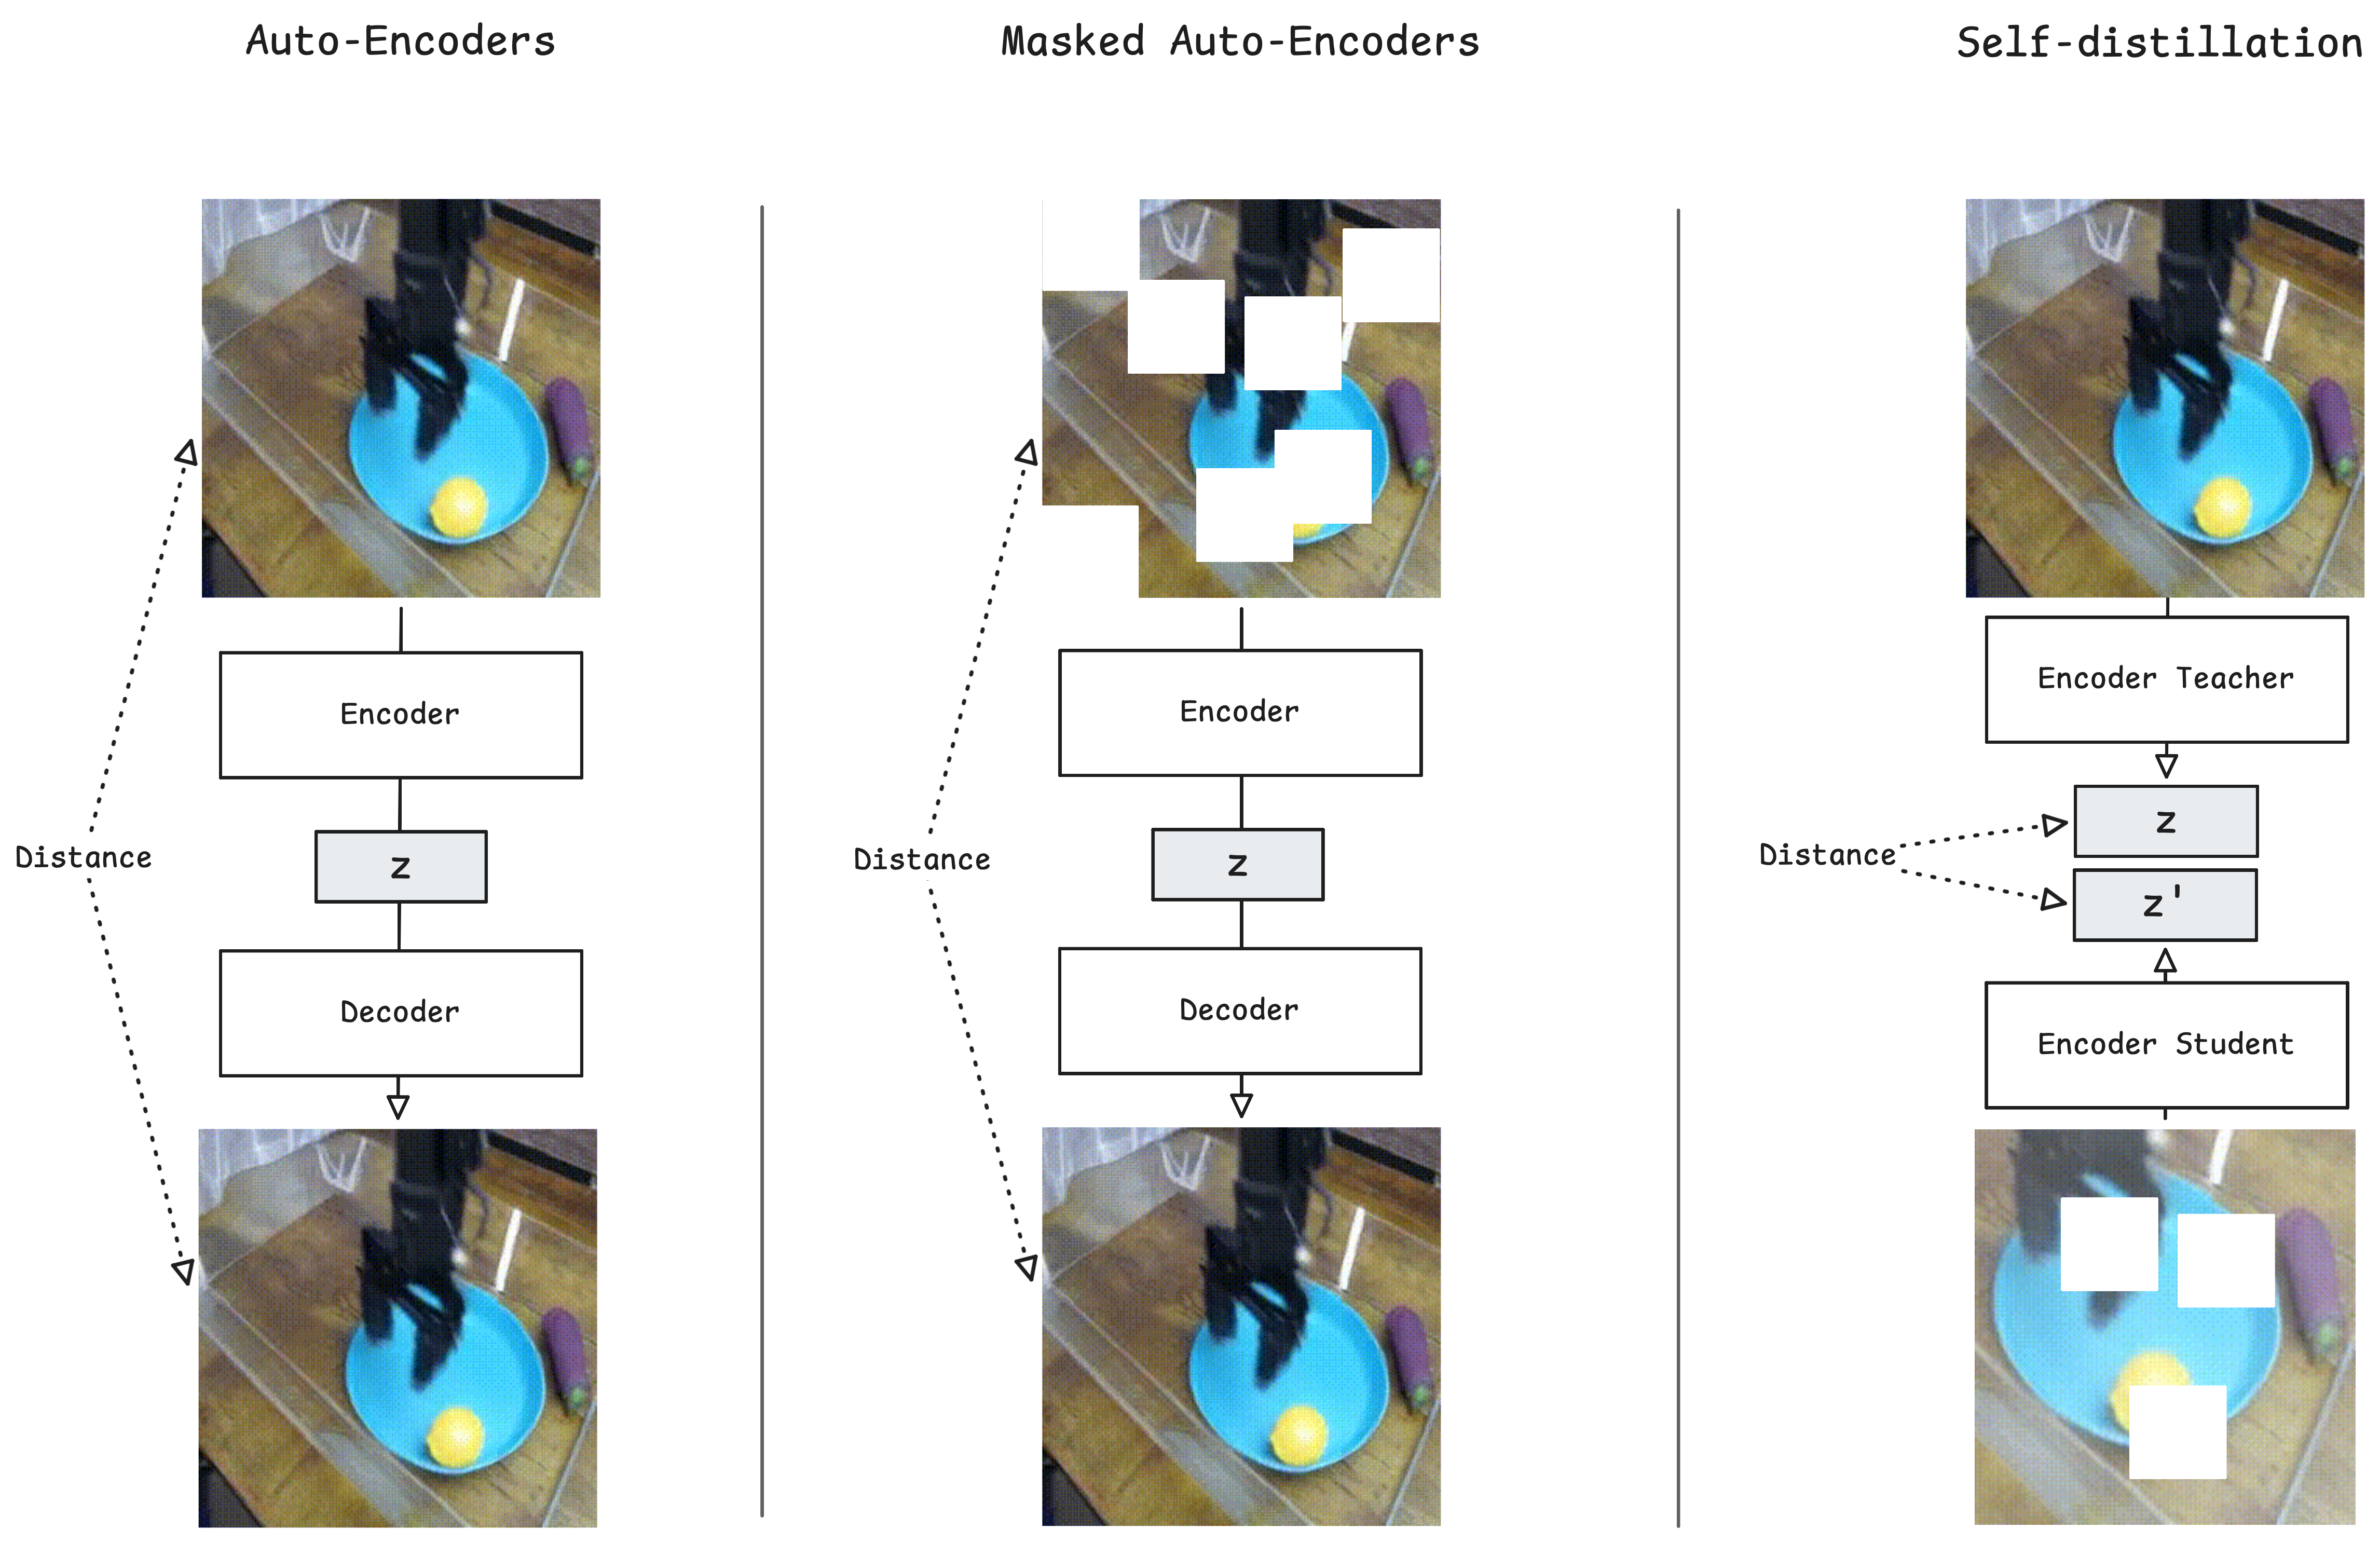
\includegraphics[width=0.9\textwidth]{images/imageencoders.png}
    \caption{Three common objectives for learning image representations: auto-encoding, masked auto-encoding, and self-distillation. The encoder maps an image to a latent representation $z$, the decoder reconstructs pixels from that representation, and in self-distillation a student encoder is trained to match the representation produced by a teacher encoder.}
    \label{fig:encoder-objectives}
\end{figure}

\paragraph{Auto-encoders.}
Auto-encoder-style models compress the entire input image into a bottleneck representation and train a decoder to reconstruct the original observation; variational autoencoders are a representative example of this family \cite{kingma2013vae}. Because the bottleneck has substantially lower dimension than the image, the model cannot simply copy every pixel and must instead encode features that are useful for reconstructing the scene, such as objects, spatial layout, and coarse appearance. Their objective rewards representations that preserve as much information as possible for pixel-level recovery. As a result, they often encode fine texture, color, and local appearance cues in addition to global scene structure. This can be useful when dense reconstruction quality matters, but it also means that the latent space may devote substantial capacity to details that are visually accurate yet irrelevant for planning. Two images that correspond to the same physical state can still appear far apart in the latent space if they differ in illumination, texture, or other superficial factors. This kind of reconstruction-based bottleneck is also widely used in modern video generation: recent systems such as Wan compress video with a VAE and train a diffusion transformer in the resulting latent space rather than synthesizing every pixel directly \cite{wan2025wan}.

\paragraph{Masked auto-encoders.}
Masked auto-encoders (MAEs) keep the reconstruction objective but make it harder and more structured: a large fraction of image patches is hidden, and the model must infer the missing content from the visible context \cite{he2021mae}. This changes what the encoder is encouraged to learn. Instead of merely compressing the whole image, the model must reason about larger-scale spatial organization, object parts, and contextual relationships in order to fill in the masked regions. Consequently, MAE features are often more semantically organized and more efficient than those learned by full-image reconstruction alone. However, the supervision signal is still ultimately based on reconstructing pixels, so the learned space remains partially tied to appearance fidelity rather than being optimized directly for semantic state similarity.

\paragraph{Self-distillation.}
Self-distillation removes the pixel decoder and supervises the representation directly in feature space. A teacher network encodes one view of an image, while a student network is trained to produce a matching representation from another augmented or partially masked view of that same image \cite{oquab2023dinov2}. The objective therefore encourages feature consistency across views, rather than accurate pixel reconstruction. This produces representations that are more invariant to nuisance changes such as color shifts, crops, and texture variation, while still retaining information about objects, layout, and scene semantics. For robotics, this is especially attractive because distances in the latent space are more likely to reflect whether two observations correspond to the same task-relevant state, rather than whether they are pixel-wise similar.

\vspace{1em}
These three objectives therefore emphasize different properties of the learned representation: auto-encoders prioritize information preservation, masked auto-encoders strengthen contextual reasoning, and self-distillation most directly promotes semantic invariance. For downstream planning, the latter property is particularly important because the world model should compare states based on controllable structure and affordances, not only on appearance.

DINOv2 is a strong example of a vision foundation model trained with large-scale self-supervision to produce robust, transferable visual features. It operates on image patches and uses a self-distillation objective, so representations from masked or augmented views are aligned in feature space rather than decoded back into pixels. This encourages object- and scene-level semantics to emerge directly in the encoder. The resulting patch-level features generalize across datasets and tasks and can be used without fine-tuning as a compact semantic state representation, which is well aligned with robotics needs \cite{oquab2023dinov2}. Figure~\ref{fig:dinov2-pca} illustrates this patch-level semantic organization with a PCA visualization of DINOv2 features.

\begin{figure}[htbp]
    \centering
    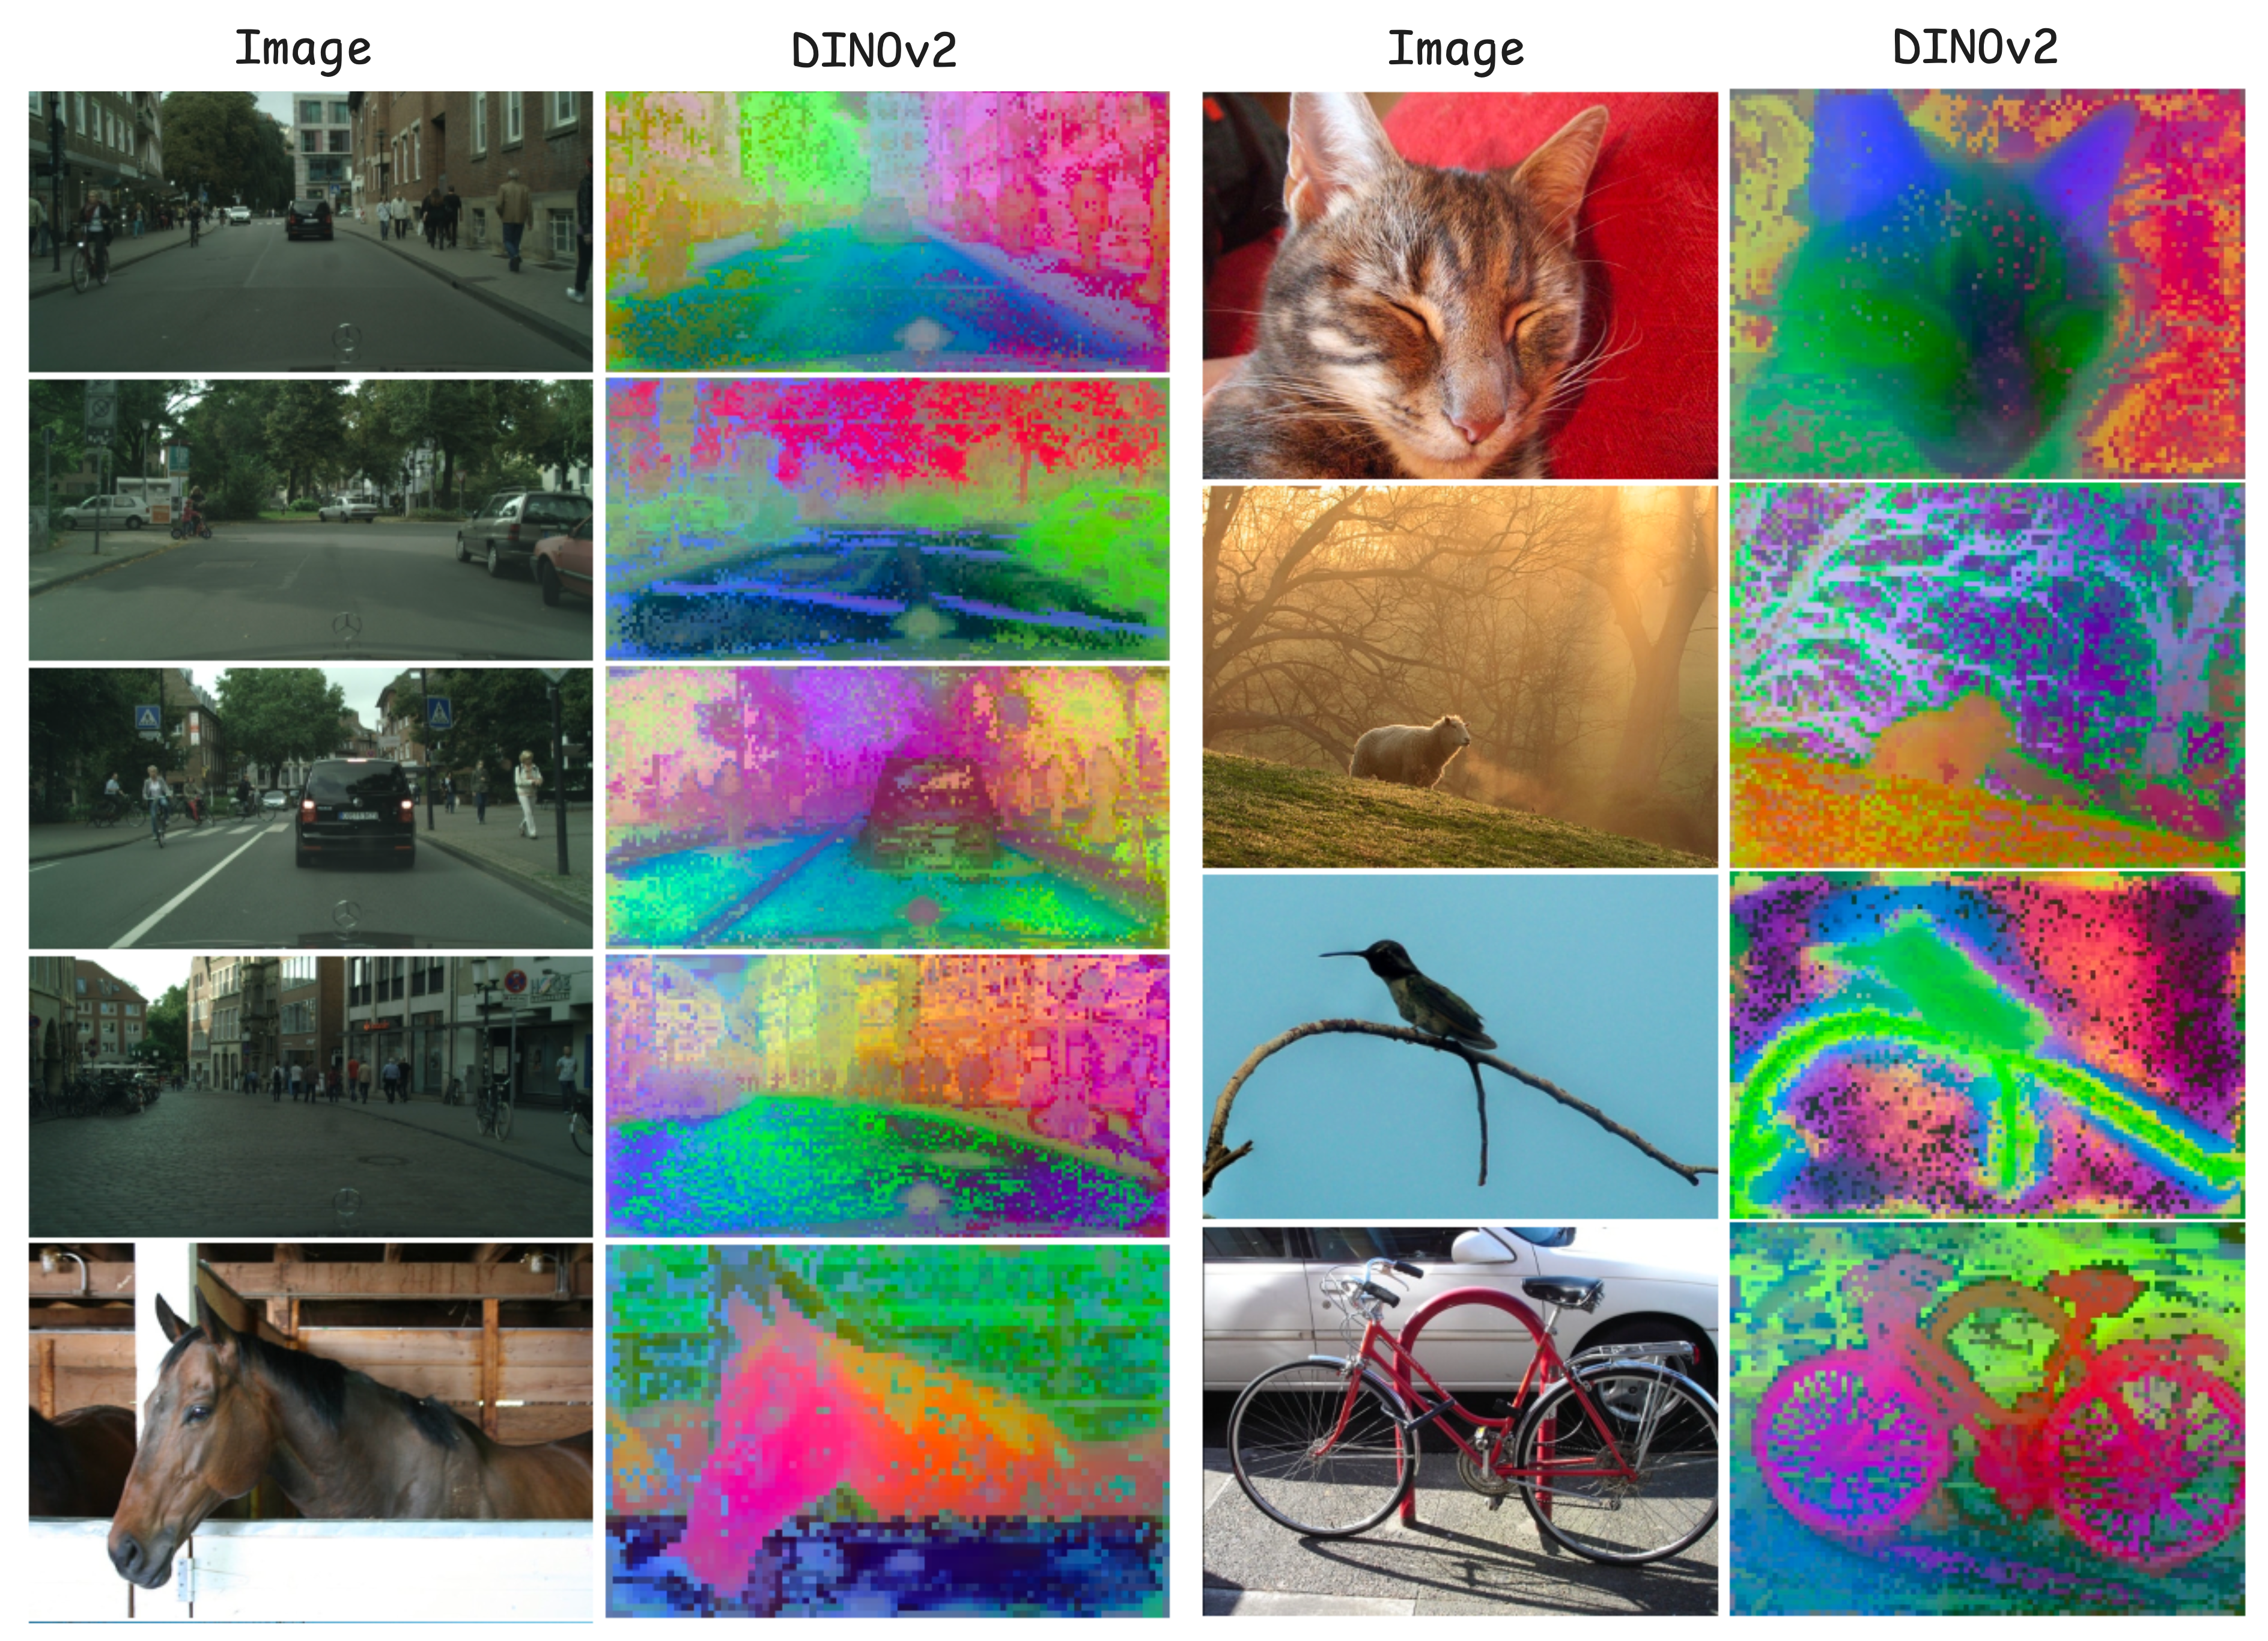
\includegraphics[width=0.8\textwidth]{images/dinov2.png}
    \caption{PCA visualization of DINOv2 patch features, adapted from Mur-Labadia et al.\ \cite{murlabadia2026vjepa21}. The high-dimensional feature vector at each image patch is projected to three principal components and displayed as RGB colors. Similar colors indicate patches with similar learned representations, showing that DINOv2 features often group coherent objects and scene regions even without pixel-level labels.}
    \label{fig:dinov2-pca}
\end{figure}

DINO-WM \cite{zhou2024dinowm} builds directly on this idea by learning a deterministic world model in the frozen DINOv2 feature space rather than in pixels. Given the current DINO patch features and an action, its dynamics model predicts the next latent state, so the model learns how the scene should evolve without reconstructing the image itself. Planning is then performed by optimizing action sequences whose predicted future features approach a desired goal feature state. Because the representation is semantically structured, distances between latent states are meaningful and provide a principled way to compare visual states for model-based planning \cite{zhou2024dinowm}. More broadly, this line of work suggests that the quality of a world model depends not only on the dynamics architecture, but also on whether its state space is aligned with task-relevant semantics.

\section{Flow Matching Generative Objectives}
The previous section argued that vision foundation models provide useful semantic state spaces for robotics. By encoding images into patch-level features, they can reduce sensitivity to nuisance variation such as lighting, texture, and small appearance changes. However, this abstraction does not remove the uncertainty inherent in predicting the future. Even in a semantic feature space, the same current state can be followed by many plausible continuations: a hand may move toward different objects, an occluded object may reappear in different locations, or a robot action may lead to slightly different contact outcomes. A world model therefore still needs a generative objective that can represent temporal stochasticity rather than only predict one average next state.

\paragraph{Why deterministic prediction fails.}
The central difficulty in video prediction is that the future is only partially determined by the past. Some aspects of the next frame are predictable from the scene history, such as object continuity, coarse motion, and physical constraints. Other aspects are inherently uncertain or simply unobserved: a hand may reach for one of several objects, an occluded object may reappear in multiple plausible places, or a bird may enter the frame from many possible directions. A learning objective that asks the model to output a single next frame therefore faces a mismatch with the data: the training target is not one deterministic continuation, but one sample from a conditional distribution of plausible futures.

This mismatch explains why simple deterministic regression is often inadequate for video dynamics. If a model is trained with a pointwise loss such as mean squared error, the optimal prediction for a multi-modal target distribution is the conditional mean. For image or video data, that mean may correspond to no physically realistic future at all. Instead of choosing one plausible outcome, the model averages several of them, which appears visually as blur, ghosting, or washed-out motion. The problem is not only cosmetic. A planner that relies on such averages receives dynamics predictions that are less semantically faithful and less useful for choosing actions.

To avoid this collapse, the model should learn the conditional distribution over future states rather than a single point estimate. Flow matching provides a practical way to model such distributions for high-dimensional continuous signals such as images, videos, or latent feature sequences \cite{lipman2023flowmatching}. Instead of asking the network to directly output the final future state, flow matching trains it to describe how a simple random sample should move toward a realistic data sample.

\paragraph{Flow matching.}
The idea of flow matching is to view generation as a transport problem. One starts from a simple distribution that is easy to sample from, such as Gaussian noise, and learns a continuous path that carries those noisy samples toward the data distribution. At any intermediate time along this path, the model receives a partially transported sample and predicts a velocity: the direction and speed in which that sample should move next. After training, generation begins from noise and repeatedly follows the learned velocity field until the sample reaches a realistic image, video, or latent feature state. Figure~\ref{fig:flow-matching} illustrates this straight interpolation view of flow matching.

\begin{figure}[htbp]
    \centering
    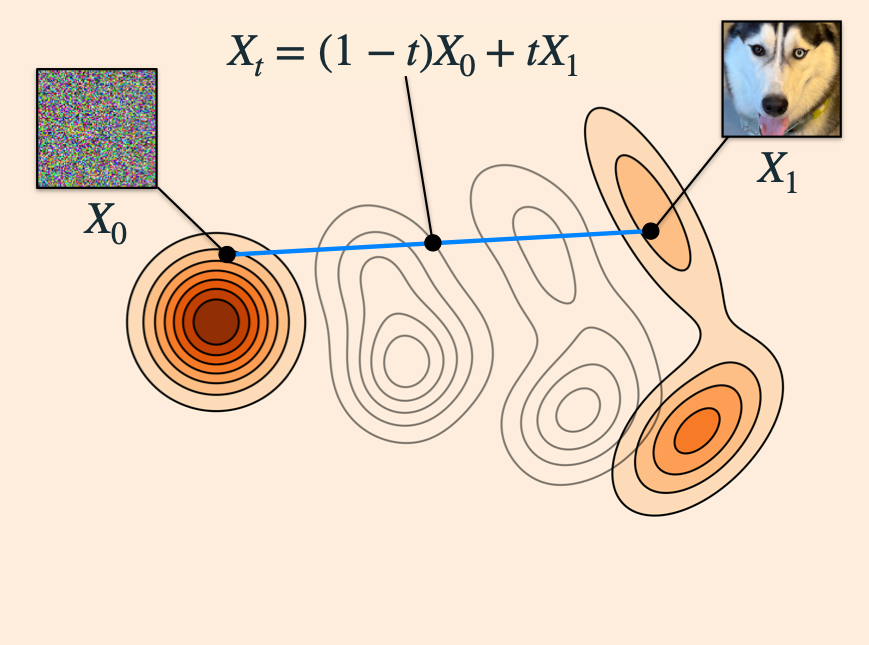
\includegraphics[width=0.5\textwidth]{images/flow_matching.png}
    \caption{Illustration of the flow matching straight interpolation path between a noise sample $X_0$ and a data sample $X_1$, adapted from Lipman et al.\ \cite{lipman2024flowmatchingguidecode}. Intermediate states $X_t = (1-t)X_0 + tX_1$ define training points along the path, and the model learns the velocity field that transports samples from the noise distribution toward the data distribution.}
    \label{fig:flow-matching}
\end{figure}

This framing is useful because the model does not need to memorize one fixed output for each input. Instead, different noise samples can be transported into different plausible futures, while conditioning information such as past frames, semantic latent states, or robot actions guides which futures are appropriate for the current context. For a world model, this means the same observed state can produce several possible next states without averaging them together. The learned vector field describes the dynamics of generation, while the conditioning context anchors those dynamics to the scene history and the proposed actions.

Rectified flow is a particularly simple and influential flow-based formulation \cite{liu2022rectifiedflow}. It encourages the learned transport paths to be as straight as possible between noise and data, which can make numerical integration easier and reduce the number of inference steps required to obtain high-quality samples. In practice, this matters because iterative generation can be computationally expensive. Straighter paths can therefore preserve the benefits of distributional modeling while making sampling more efficient.

\paragraph{Why this matters for world models.}
For videos, distributional modeling is essential. Real scenes contain stochastic interactions, partial observability, and many locally unpredictable details, yet a useful model must still produce samples that respect global structure and physical constraints. Flow matching is well suited to this setting because it turns high-dimensional generation into a sequence of simpler transport steps while retaining multi-modality. In a semantic world model, the same principle can be applied directly in representation space: instead of transporting noise toward raw pixels, the model can transport noisy latent features toward plausible future semantic states. The RAE work demonstrates this idea for image generation by training diffusion transformers with flow matching inside latent spaces produced by pretrained representation encoders such as DINOv2 \cite{dt_rae2025}. Because these latents are much higher-dimensional than conventional VAE bottlenecks, that recipe normalizes representation patches and uses a dimension-aware noise schedule; the corresponding choices used in this thesis are described in Chapter 3. This fits naturally with vision foundation models, because the encoder supplies a semantic latent space that is less sensitive to small pixel-level perturbations and other nuisance variation, while the flow objective models uncertainty in how that state may evolve over time.

\section{World Models, Imagined Rollouts, and Planning}
\subsection{World Models as Predictive Simulators}
A world model is a learned predictive model of how the environment evolves \cite{ha2018worldmodels,hafner2019planet}. In the robotics setting, it approximates how future observations or latent states change as a function of the current history and candidate actions. Once such a model is available, it becomes possible to plan in imagination: instead of trying many actions on the physical robot, the agent can test them inside the learned model and evaluate their predicted consequences before acting \cite{ha2018worldmodels,hafner2019dreamer,hafner2020dreamerv2,hafner2023dreamerv3}.

The basic operation that makes this possible is the imagined rollout. Starting from the current observation, the model predicts the next state under a candidate action, then uses that predicted state as part of the context for the following prediction. Repeating this process produces an imagined trajectory. In the ideal case, such a rollout would be a faithful sample from the true environment dynamics: every generated state would remain physically plausible, semantically consistent, and correctly conditioned on the proposed actions. This is the sense in which a world model acts as a simulator for planning. In practice, however, this recursive generation is also where the main failure mode appears.

\subsection{Planning with Imagined Trajectories}
Imagined rollouts are especially useful for goal-directed behavior. Given the current observation and a desired goal state, the planner proposes candidate action sequences, rolls them out through the world model, and scores the resulting trajectories according to how close they come to the goal. The search over actions is therefore grounded in predicted future outcomes rather than in a purely reactive mapping from observations to actions. Figure~\ref{fig:latent-mpc-rollout} summarizes this latent-space planning loop.

\begin{figure}[htbp]
    \centering
    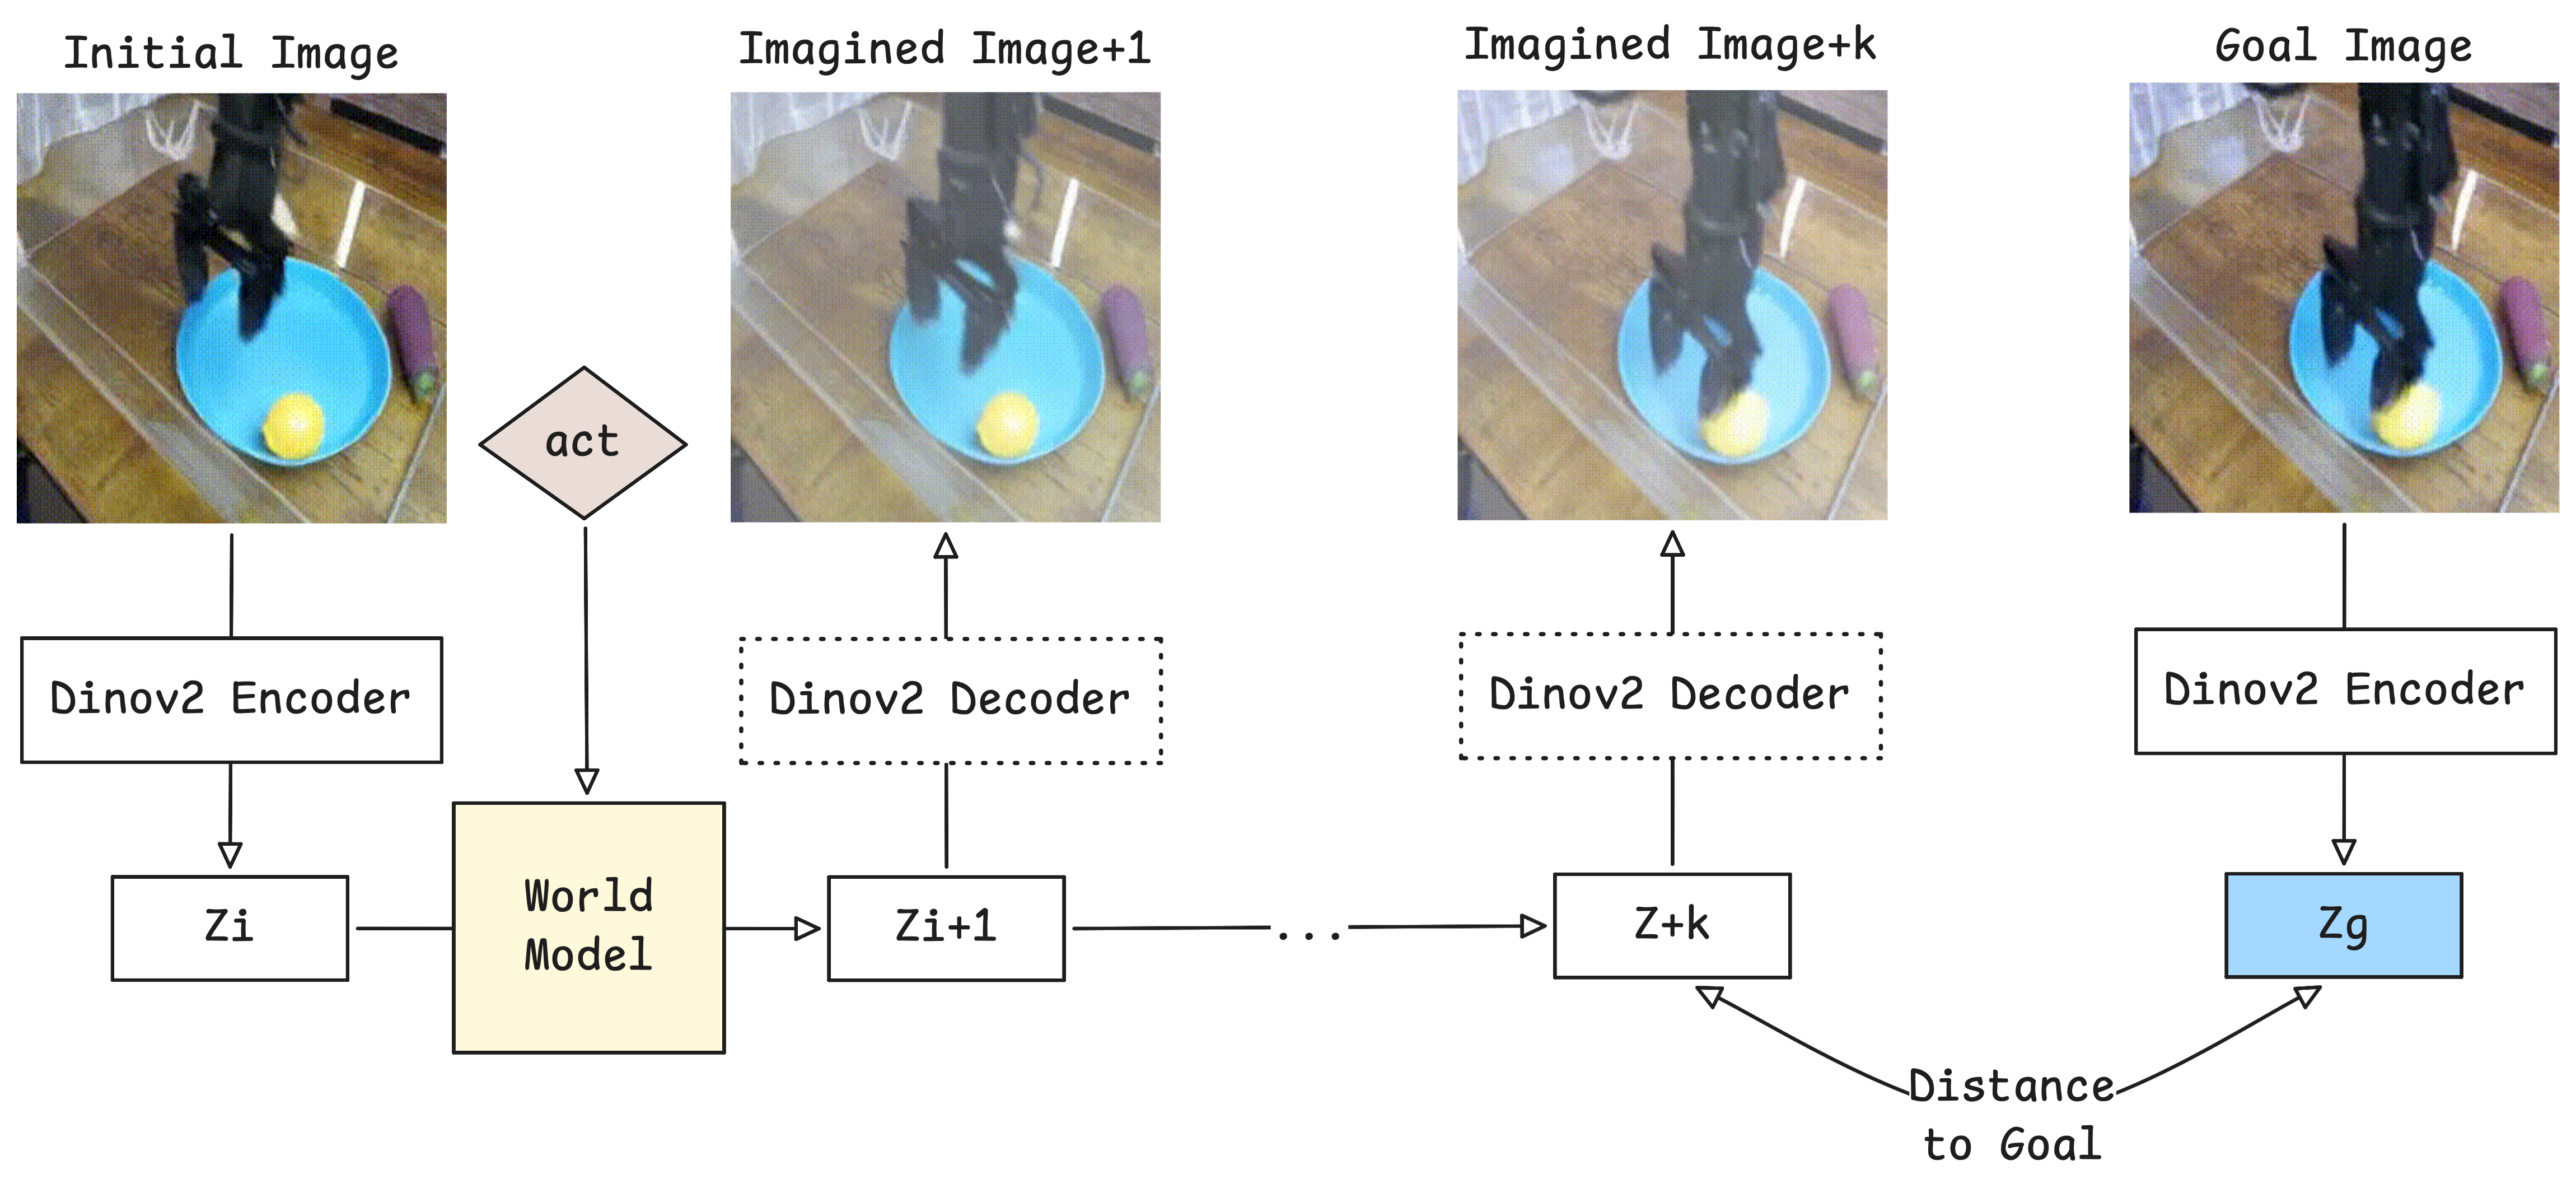
\includegraphics[width=1.0\textwidth]{images/worldmodel.png}
    \caption{Latent-space goal-directed planning with a learned world model. The current and goal observations are encoded with DINOv2, candidate action sequences are rolled out in latent space, optional decoder reconstructions visualize imagined futures, and the rollout with the smallest latent distance to the goal is selected.}
    \label{fig:latent-mpc-rollout}
\end{figure}

The usefulness of a world model for planning depends on both its state representation and its uncertainty modeling. The representation should preserve task-relevant semantics so that distances between predicted and goal states are meaningful. The dynamics objective should preserve multiple plausible futures rather than collapse them into an average. This is why semantic encoders and flow-based objectives fit naturally together: the first provides a state space aligned with control, while the second provides a way to model uncertainty in how that state may evolve.

In practice, planning also requires an optimizer over action sequences. A common choice is the Cross-Entropy Method (CEM), a population-based optimizer that alternates between sampling candidate action sequences, evaluating them under the learned model, selecting an elite subset, and refitting a sampling distribution around those elites \cite{botev2013cem}. This is attractive because the planning objective can remain non-convex and need not be analytically differentiable. In representation-space world models such as DINO-WM, the cost can be defined directly as the latent distance between the predicted rollout and the encoded goal state \cite{zhou2024dinowm}. The resulting planner is simple: encode the current image and the goal image, imagine candidate futures, and score them in latent space.

\subsection{Long-Horizon Rollout Drift}
The recursive structure of imagined rollouts creates a training-inference mismatch. Autoregressive world models are usually trained on ground-truth prefixes: when predicting the next frame or latent state, their conditioning history comes from real data. At deployment, however, the model is conditioned on its own previous predictions. This mismatch is known as exposure bias in sequence modeling: once the model makes a small error, the next prediction is conditioned on an input it never saw during training, and the resulting errors can accumulate rapidly along the generated sequence \cite{bengio2015scheduled}.

For video world models, this means that one-step accuracy is not enough. A model may predict plausible short-term transitions but still drift when rolled out over many steps, because each generated state becomes part of the next input context. Small local errors can gradually push the imagined trajectory off the data manifold, causing long rollouts to become less realistic, less temporally coherent, and less useful for downstream planning. This is particularly damaging for planning, because candidate actions are scored by their predicted futures, so drift can make the planner prefer actions that look good only under a corrupted imagined trajectory.

\subsection{Diffusion Forcing as a Remedy}
Diffusion Forcing is designed to address this failure mode while retaining causal sequence generation \cite{chen2024diffusionforcing}. The core idea is to train on sequences in which each token is corrupted with its own noise level, rather than assigning a single global diffusion timestep to the whole sequence. Low-noise tokens behave like trusted context, high-noise tokens behave like uncertain future states, and the model learns to denoise the latter conditioned on the former. Standard next-token prediction appears as one limiting case, where the past is effectively clean and only the next token is strongly corrupted. Full-sequence diffusion appears as the opposite extreme, where all tokens share the same noise level. Figure~\ref{fig:diffusion-forcing} contrasts this setup with standard teacher forcing.

\begin{figure}[htbp]
    \centering
    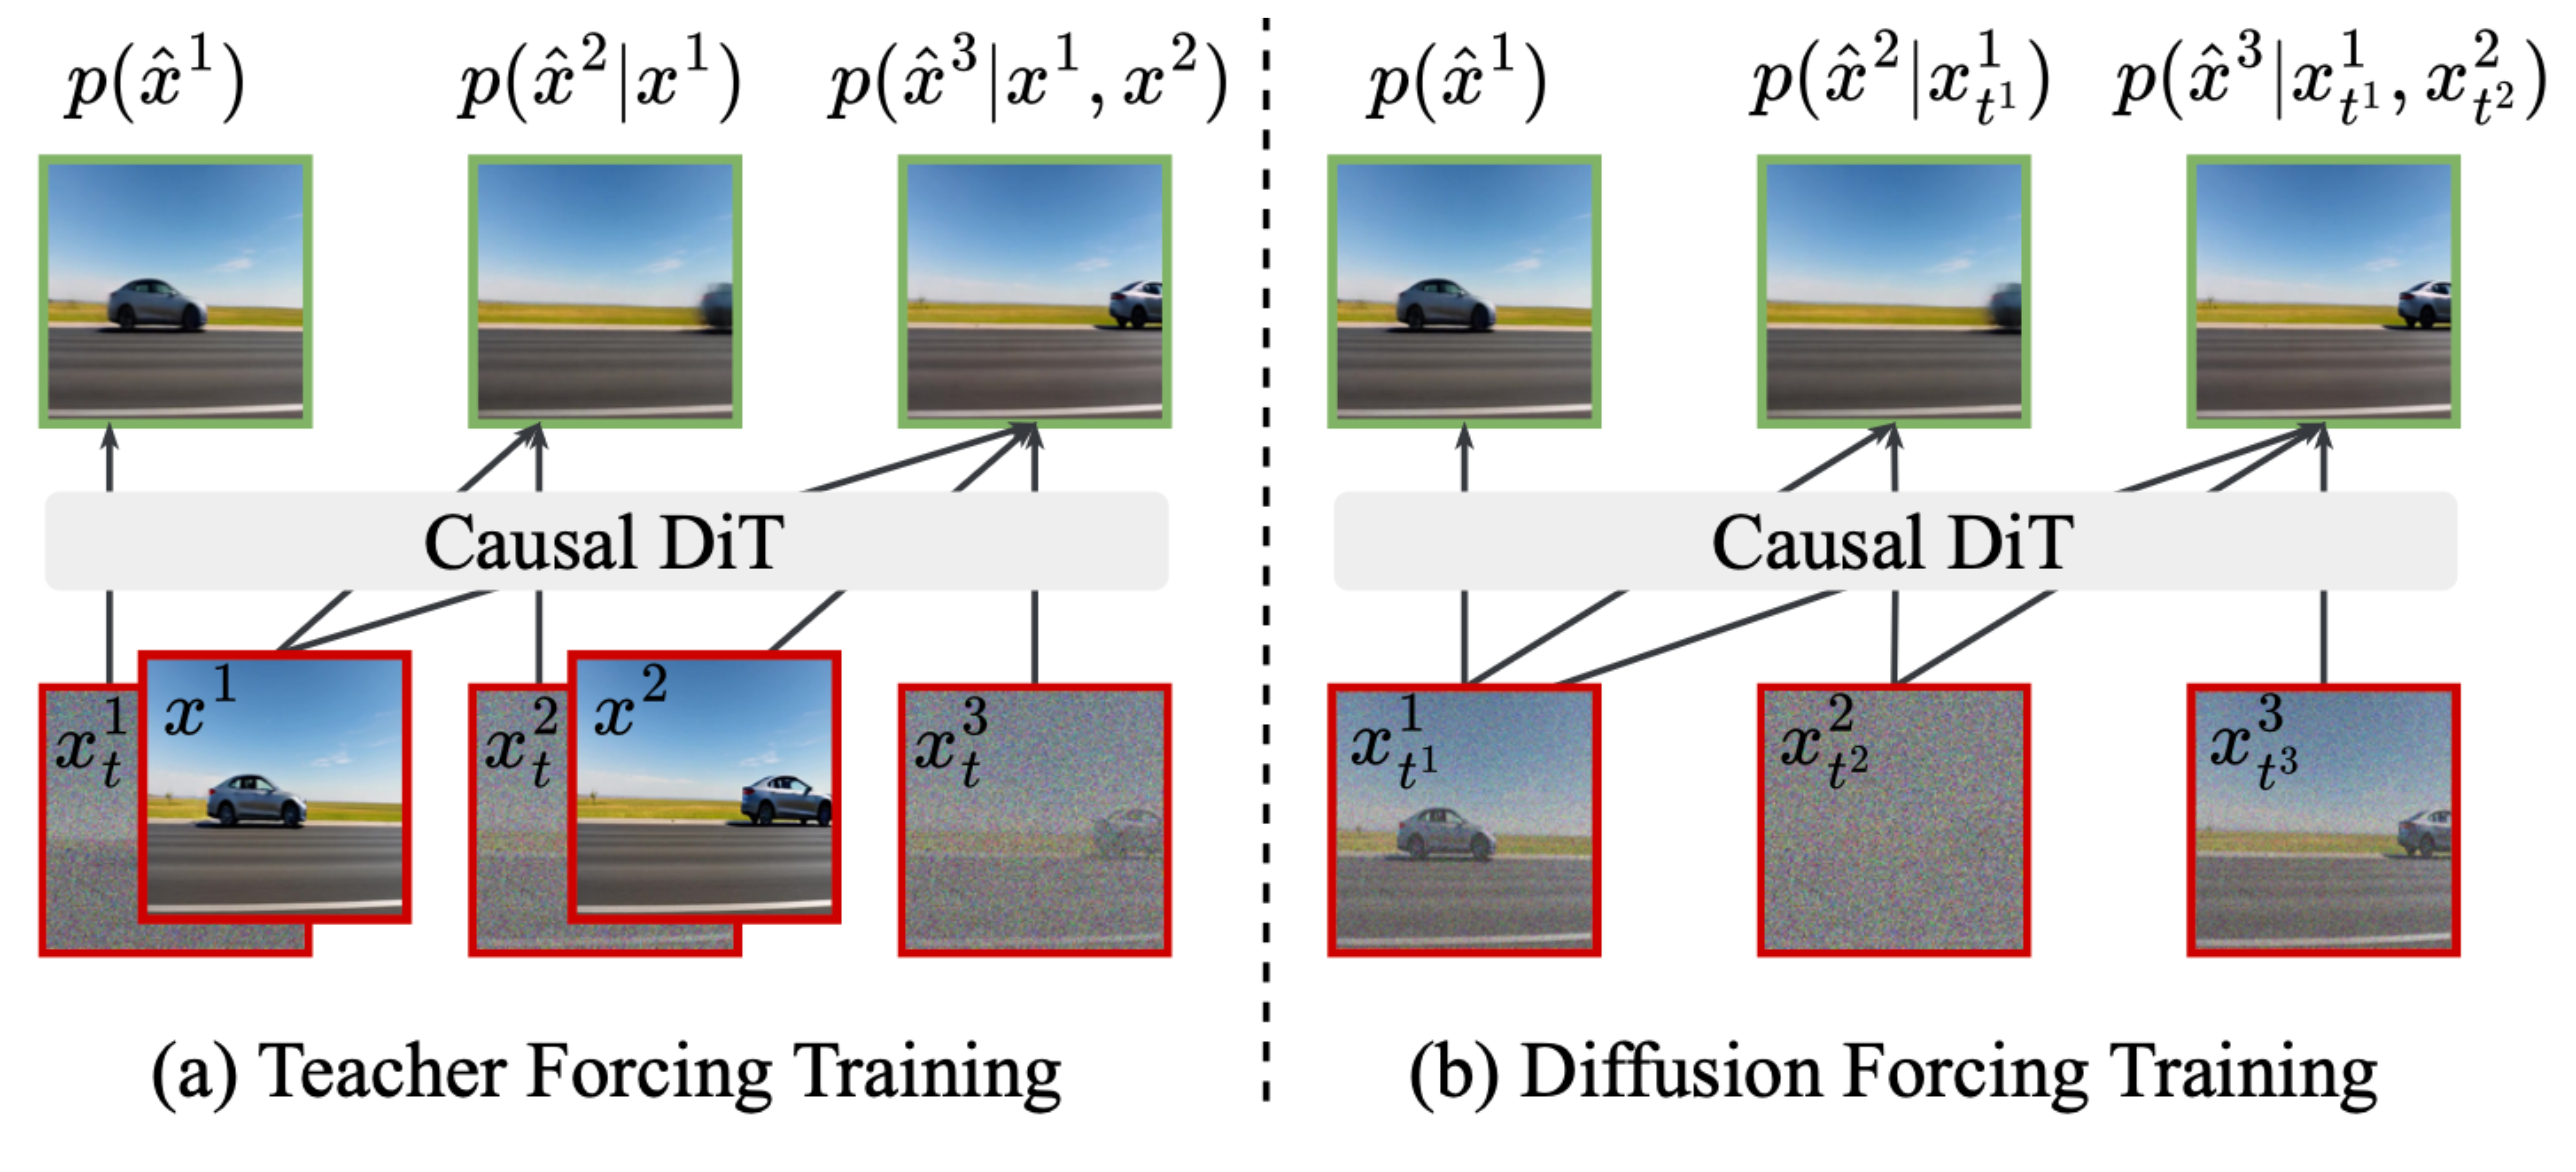
\includegraphics[width=0.9\textwidth]{images/diffusion_forcing.png}
    \caption{Teacher forcing compared with Diffusion Forcing, adapted from Huang et al.\ \cite{huang2025selfforcing}. In teacher forcing, future predictions are conditioned on clean ground-truth past frames during training. In Diffusion Forcing, different tokens are corrupted by different noise levels, so the model learns to denoise uncertain future tokens while conditioning on partially clean or partially corrupted context.}
    \label{fig:diffusion-forcing}
\end{figure}

This per-token noising scheme can be understood as \emph{noise as masking}. Instead of conditioning only on perfect histories, the model is trained on a continuum of partially corrupted prefixes. As a result, it learns to recover plausible futures even when the conditioning history is imperfect, which is precisely the situation encountered during long-horizon rollout when earlier predictions are no longer exact. Chen et al.\ show that this formulation combines the variable-horizon, causal advantages of autoregressive models with the sequence-level guidance capabilities of diffusion models, and empirically supports rollouts beyond the training horizon where conventional baselines diverge \cite{chen2024diffusionforcing}.

For robotics, this matters in two ways. First, more stable imagined rollouts make planning more reliable because candidate action sequences are evaluated on futures that drift less severely over time. Second, because future tokens remain diffusion variables during sampling, the same model still supports sequence-level guidance and planning rather than committing too early to a single deterministic continuation. Diffusion Forcing therefore fits naturally into semantic world models: it preserves causal action conditioning while making long-horizon imagination more robust.

\subsection{Alternative World Models for Robot Planning}
World models for robotics differ along several important axes: what they predict, what data they require, and how the learned model is used for decision making. Some predict future pixels directly, others learn compact latent states jointly with the dynamics model, and more recent methods use pretrained visual representations or large generative video models. These choices are not merely implementation details. They determine whether planning is performed in image space or representation space, whether passive video can be exploited easily, and whether the model is optimized for online control, offline planning, or policy learning in imagination.

An early and influential line of robot world models predicts future images directly. Deep Visual Foresight combines action-conditioned video prediction with model predictive control so that a robot can evaluate candidate pushing actions by imagining their visual consequences \cite{finn2016visualforesight}. Later visual MPC work extended this approach to user-specified visual goals and broader real-world manipulation settings \cite{ebert2018visualforesight}. Pixel-space prediction has the advantage that the model output is directly interpretable and supervision can be obtained from raw robot videos without manually labeled states. Its limitation is that planning must operate in a very high-dimensional space where appearance details such as color, texture, or lighting are modeled together with task-relevant motion.

A second family learns compact latent dynamics models rather than predicting pixels directly at decision time. The world-model framework of Ha and Schmidhuber demonstrated that a compressed latent simulator can support downstream control in imagination \cite{ha2018worldmodels}. PlaNet learned stochastic recurrent state-space dynamics from pixels and selected actions by planning over imagined latent trajectories \cite{hafner2019planet}. The Dreamer family used related latent dynamics models to train actor-critic behavior policies inside imagined rollouts, improving sample efficiency and scaling across increasingly diverse domains \cite{hafner2019dreamer,hafner2020dreamerv2,hafner2023dreamerv3}. These methods make planning or policy learning more efficient by compressing the visual stream into a learned state, but the representation is optimized jointly with the control objective rather than fixed to a pretrained semantic space.

Frozen semantic-feature world models take a different position in this design space. DINO-WM predicts future DINOv2 patch features instead of reconstructing pixels, and uses the distance between predicted and goal features for zero-shot action-sequence optimization \cite{zhou2024dinowm}. This shows that planning can be effective without photorealistic image prediction when the representation already organizes observations by task-relevant visual semantics. DINO-WM is therefore the closest precedent to this thesis: both approaches use pretrained semantic features as the state space for visual planning. The main difference is that the present work studies a diffusion-based sequence model trained with mixed action-labeled robot data and action-free video, rather than a conventional predictive model trained only on action-compatible trajectories.

Recent diffusion-based alternatives have explored a different route for using large video corpora in robotics. AVID adapts pretrained image-to-video diffusion models into action-conditioned world models by learning an adapter from a small action-labeled dataset \cite{rigter2024avid}. Unified World Models encode observations into VAE video latents and model those latents together with actions inside one transformer, allowing the same architecture to represent forward dynamics, inverse dynamics, policy prediction, and video generation while also learning from action-free video \cite{zhu2025uwm}. These works are closely aligned with the motivation of using abundant video beyond expert robot demonstrations, but they primarily operate through diffusion over video latents rather than through a frozen semantic feature space dedicated to latent planning. Table~\ref{tab:related-world-model-families} summarizes these neighboring world-model families.

\begin{table}[h]
\caption{Comparison of representative world-model families relevant to robotic planning. The main trade-offs concern the prediction space, the kind of supervision required, and whether the model is used for pixel-space MPC, latent planning, policy learning, or semantic goal-conditioned optimization.}
\label{tab:related-world-model-families}
\begin{center}
\small
\begin{tabular}{@{}L{0.18\textwidth} L{0.22\textwidth} L{0.22\textwidth} L{0.25\textwidth}@{}}
\toprule
\textbf{Work family} & \textbf{Prediction space} & \textbf{Typical data regime} & \textbf{Use at decision time} \\
\midrule
Visual foresight / visual MPC & Future pixels or pixel motion & Action-labeled robot interaction video & Model predictive control over imagined image futures \\
PlaNet / Dreamer-style latent models & Learned compact latent state & Environment interaction with rewards or observations & Latent planning or policy learning in imagination \\
DINO-WM & Frozen DINOv2 patch features & Offline action trajectories & Goal-conditioned action-sequence optimization in semantic feature space \\
Diffusion foundation-style models such as AVID and Unified World Models & Video latents, with action tokens when modeled jointly & Pretrained video priors plus robot data, with optional action-free video & Goal-conditioned action-sequence optimization over predicted futures \\
\midrule
This thesis & Frozen DINOv2 patch features & Mixed passive video and action-labeled robot data & Latent-space CEM planning with diffusion-based rollouts \\
\bottomrule
\end{tabular}
\end{center}
\end{table}

\section{Positioning of This Thesis}
The comparison above places this thesis at the intersection of three ideas that prior work has usually emphasized separately: semantic visual representations from self-supervised encoders \cite{oquab2023dinov2}, world models for imagination-based control \cite{ha2018worldmodels,hafner2019planet,hafner2023dreamerv3}, and flow-based objectives for modeling multi-modal sequential data \cite{lipman2023flowmatching,liu2022rectifiedflow}. The central design choice is to retain the semantic planning space of DINO-WM while adopting a diffusion-style dynamics objective and a mixed-data training regime that can incorporate action-free video.

This makes the thesis distinct from several neighboring approaches. Compared with visual-foresight methods, it does not plan from predicted pixels, but from predicted semantic latent states. Compared with Dreamer-style model-based reinforcement learning, it uses a fixed pretrained representation and focuses on visual goal-conditioned planning rather than learning a reward-conditioned behavior policy. Compared with DINO-WM, it asks whether the same semantic planning principle can be combined with per-frame diffusion corruption and heterogeneous video training. Compared with recent diffusion world models such as AVID and Unified World Models, it studies whether the benefits of large video data can be obtained in a frozen representation space rather than by modeling video latents directly. The exact architecture, data pipeline, training configuration, and evaluation protocol are described in the methodology and experiments chapters.

%%==========================================================================
%% CHAPTER 3: METHODOLOGY
%%==========================================================================
\chapter{Methodology}

\noindent
This chapter describes how the world model is built, trained, evaluated, and used for planning. The system has four main components. First, visual observations are converted into dense DINOv2 patch features. Second, a spatial-temporal transformer is trained to denoise and predict sequences in that latent space. Third, heterogeneous video and robot datasets are loaded through a common sequence interface so that passive video and action-labeled robot data can be mixed during training. Finally, the trained model is used as a latent simulator inside a Cross-Entropy Method planner.

\section{End-to-End System}
The training pipeline is shown in Figure~\ref{fig:method-pipeline}. A video sequence is sampled from an offline dataset, transformed to the encoder resolution, and encoded frame by frame into DINOv2 latents. The clean latent sequence is then corrupted with independently sampled signal levels, and the transformer is trained to map the noised sequence back toward the clean latent states. In the figure, the different opacity levels of the latent-state icons visualize this per-frame corruption: each frame receives its own sampled noise level rather than sharing one sequence-wide level. The diagonal connections entering the temporal layer illustrate causal temporal attention: each frame may attend to itself and earlier frames, but never to future frames. The action position is always initialized with a learned base action token; when an action is available, its projected embedding is added to that base token. This allows the same sequence format to cover passive video, robot video without action conditioning, and action-conditioned robot trajectories.

\begin{figure}[H]
    \centering
    
\includegraphics[width=1.0\textwidth]{images/method_pipeline.png}
    \caption{End-to-end training method. Frames are encoded into DINOv2 patch features, corrupted according to independently sampled per-frame signal levels, and denoised by the spatial-temporal transformer. The varying opacity of the latent-state icons denotes these different frame-specific corruption levels. The diagonal temporal connections denote causal attention, so each frame can use only its own state and preceding frames, not future frames. The action position contains a learned base action token, with a projected robot action added when action conditioning is available.}
    \label{fig:method-pipeline}
\end{figure}

At evaluation and planning time, the trained transformer is rolled forward autoregressively. Observed frames are encoded as context, future frames are sampled by iterative denoising, and generated latents are fed back into the temporal cache for subsequent predictions. For planning, candidate action sequences are evaluated by comparing the terminal predicted latent state with the latent encoding of a goal image.

\section{Visual State Representation}
\subsection{Frozen DINOv2 Features}
Each observation image $I_t$ is transformed into a latent state $z_t$ using a frozen DINOv2 encoder with register tokens \cite{oquab2023dinov2,darcet2023registers}.
The encoder follows the preprocessing used by the DINO representation autoencoder (RAE) work \cite{dt_rae2025}. Images are converted to RGB tensors, resized and center-cropped to $224 \times 224$, normalized with the DINOv2 image statistics, and passed through the encoder without gradient updates. As in the RAE setup, the learned affine parameters of the final DINOv2 LayerNorm are removed, and the resulting patch features are normalized with stored mean and variance statistics computed on ImageNet. The class token and the four DINO register tokens are discarded after encoding; only the dense image patch tokens are kept. With a DINOv2 patch size of $14 \times 14$ pixels, a $224 \times 224$ image is split into a $16 \times 16$ grid, giving $16\cdot16=256$ patch tokens per frame. Each DINOv2 base patch token is a 768-dimensional feature vector, so one latent frame has shape
\begin{equation}
\label{eq:dino-latent-shape}
z_t \in \mathbb{R}^{256 \times 768}.
\end{equation}
Thus, a sequence of $T$ frames is represented as $z_{1:T} \in \mathbb{R}^{T \times 256 \times 768}$ before it enters the world model.

Using a frozen encoder is mainly a practical design choice. It avoids training a large visual backbone together with the dynamics model, makes the latent targets available without additional supervision, and gives a fixed coordinate system in which rollout errors and goal distances can be measured. A jointly trained encoder could in principle be used, but it would make the representation, the dynamics model, and the planning metric move together during training. For this thesis, the frozen DINOv2 representation keeps the world-model problem focused on learning temporal dynamics rather than learning visual features from scratch.

\subsection{Decoder for Visualization}
Although the world model operates entirely in the DINO latent space, it is very useful to visualize what its generations correspond to in image space. For this purpose, the pretrained decoder from the DINO representation autoencoder (RAE) work is used \cite{dt_rae2025}. The decoder receives predicted DINO patch features and reconstructs an RGB image. It is not used as a training loss for the world model: the dynamics loss is computed directly in latent space, and the decoder is only used for qualitative rollout videos and denoising diagnostics.
Before decoding, the RAE normalization is inverted using the same stored statistics described above. This makes the decoder a diagnostic tool for interpreting latent rollouts, not a component that changes the training objective or the planning cost.

\section{Input Sequence Construction}
Each latent frame is converted into a transformer input by concatenating the 256 DINO patch tokens with a small set of prefix tokens. These prefix tokens provide information that is not contained in the image features alone: the current diffusion signal level, the robot action when available, and learned register slots that act as frame-level workspace tokens. In the main action-capable configuration, the token order is
\begin{equation}
\label{eq:token-layout}
[\mathrm{signal},\ \mathrm{action},\ \mathrm{register}_1,\ldots,\mathrm{register}_4,\ z_{t,1},\ldots,z_{t,256}],
\end{equation}
where all tokens are projected to the transformer width before attention. The construction of each token type is described below and summarized afterward in Figure~\ref{fig:token-pipeline}.

\noindent\textbf{Signal token.}
The signal token follows the DreamerV4-style conditioning interface \cite{hafner2025dreamerv4}. The scalar signal level $s_t$ is embedded with sinusoidal features and an MLP, then inserted as a token so every transformer layer can condition on how noisy the current frame is. This is the token that tells the model whether it should treat the patch tokens as nearly clean context, heavily corrupted future state, or an intermediate case.

\noindent\textbf{Action token.}
The action token position is always initialized with a learned base action token. When an action is available for the sampled transition, the normalized 7-dimensional action vector is linearly projected to the transformer width and added to this base token. For the UR5 data, this action vector represents the relative local end-effector motion between two consecutive 5 Hz states: three translation components, three orientation components, and one gripper component. The action aligned with frame $z_t$ describes the transition from $z_{t-1}$ to $z_t$, so the first frame in a sampled sequence has no preceding transition and uses only the base action token.

\noindent\textbf{Action masking.}
When an action is unavailable or intentionally masked, no projected action vector is added, so the token remains only the learned base action token. This follows the DreamerV4 convention of giving the model an explicit token that represents missing action information \cite{hafner2025dreamerv4}. In mixed video training this is important: action-labeled robot samples and passive video samples can share the same token layout, while the model can still distinguish whether a transition is action-conditioned.

\noindent\textbf{Register tokens.}
The four register tokens are learned vectors that are inserted for every frame. They are inspired by the register-token idea in vision transformers \cite{darcet2023registers}. They give the model a small set of non-image tokens that can collect and redistribute global frame information before the output is read from the patch tokens.

\noindent\textbf{Patch tokens.}
The 256 DINO patch tokens contain the visual state. Each one starts as a 768-dimensional DINO feature vector and is projected to the transformer's internal width before attention. At the output, the model projects the patch-token states back to the DINO feature dimension. Only these patch tokens are predicted and included in the loss; the signal, action, and register tokens are internal conditioning variables.

\begin{figure}[H]
    \centering
    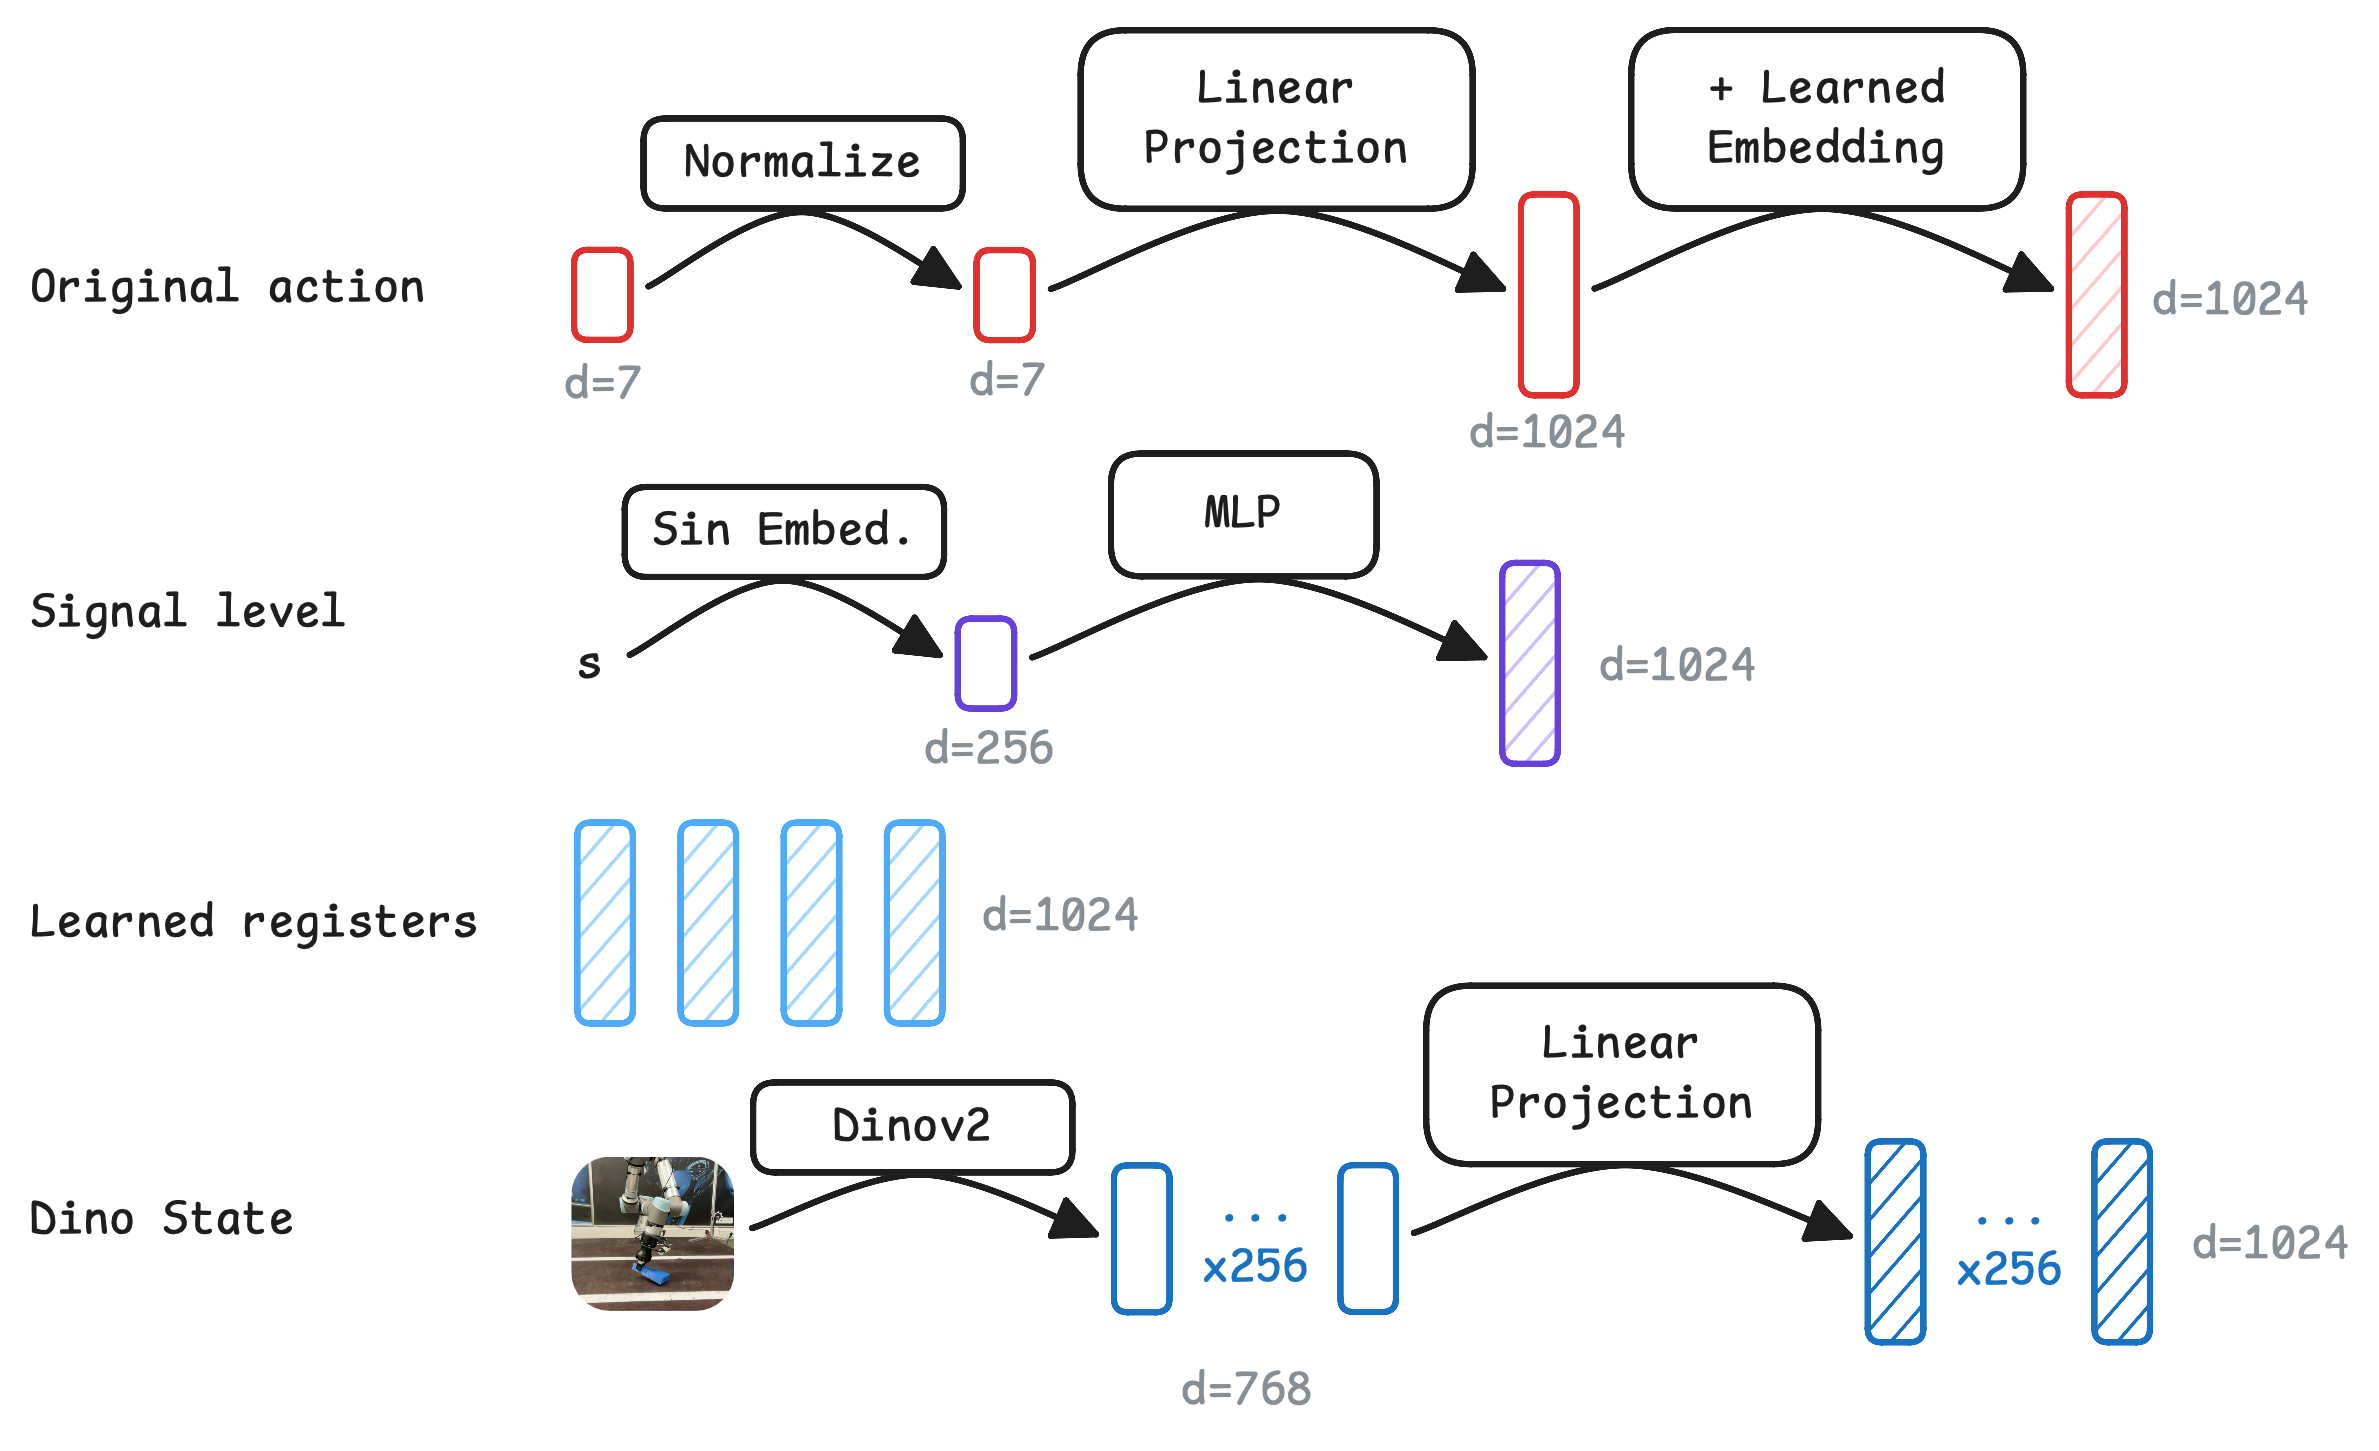
\includegraphics[width=0.95\textwidth]{images/token_pipeline.png}
    \caption{Per-frame token construction. A scalar signal level is embedded into a signal token, the learned base action token is always present and receives an added projected 7-dimensional action embedding when available, four learned register tokens provide frame-level workspace, and the 256 DINO patch tokens are projected from their 768-dimensional feature space to the transformer width.}
    \label{fig:token-pipeline}
\end{figure}

\section{Spatial-Temporal Transformer}
\subsection{Block-Causal Backbone}
The dynamics model is a block-causal transformer inspired by the scalable world-model architecture of DreamerV4 \cite{hafner2025dreamerv4}. Its role is to model a sequence of latent frames while preserving the autoregressive structure needed for rollout. The full dynamics model contains approximately 400 million trainable parameters and uses 24 blocks, model width 1024, 16 attention heads, and four learned register tokens per frame. Several stability choices are inherited from recent large transformer practice: pre-attention RMSNorm, query-key RMS normalization, rotary positional embeddings, residual scaling at initialization, SwiGLU feed-forward layers, and attention logit soft-capping. Figure~\ref{fig:token-layout-factorized-attention} shows the per-frame token layout and the factorized spatial-temporal attention pattern.

\begin{figure}[H]
    \centering
    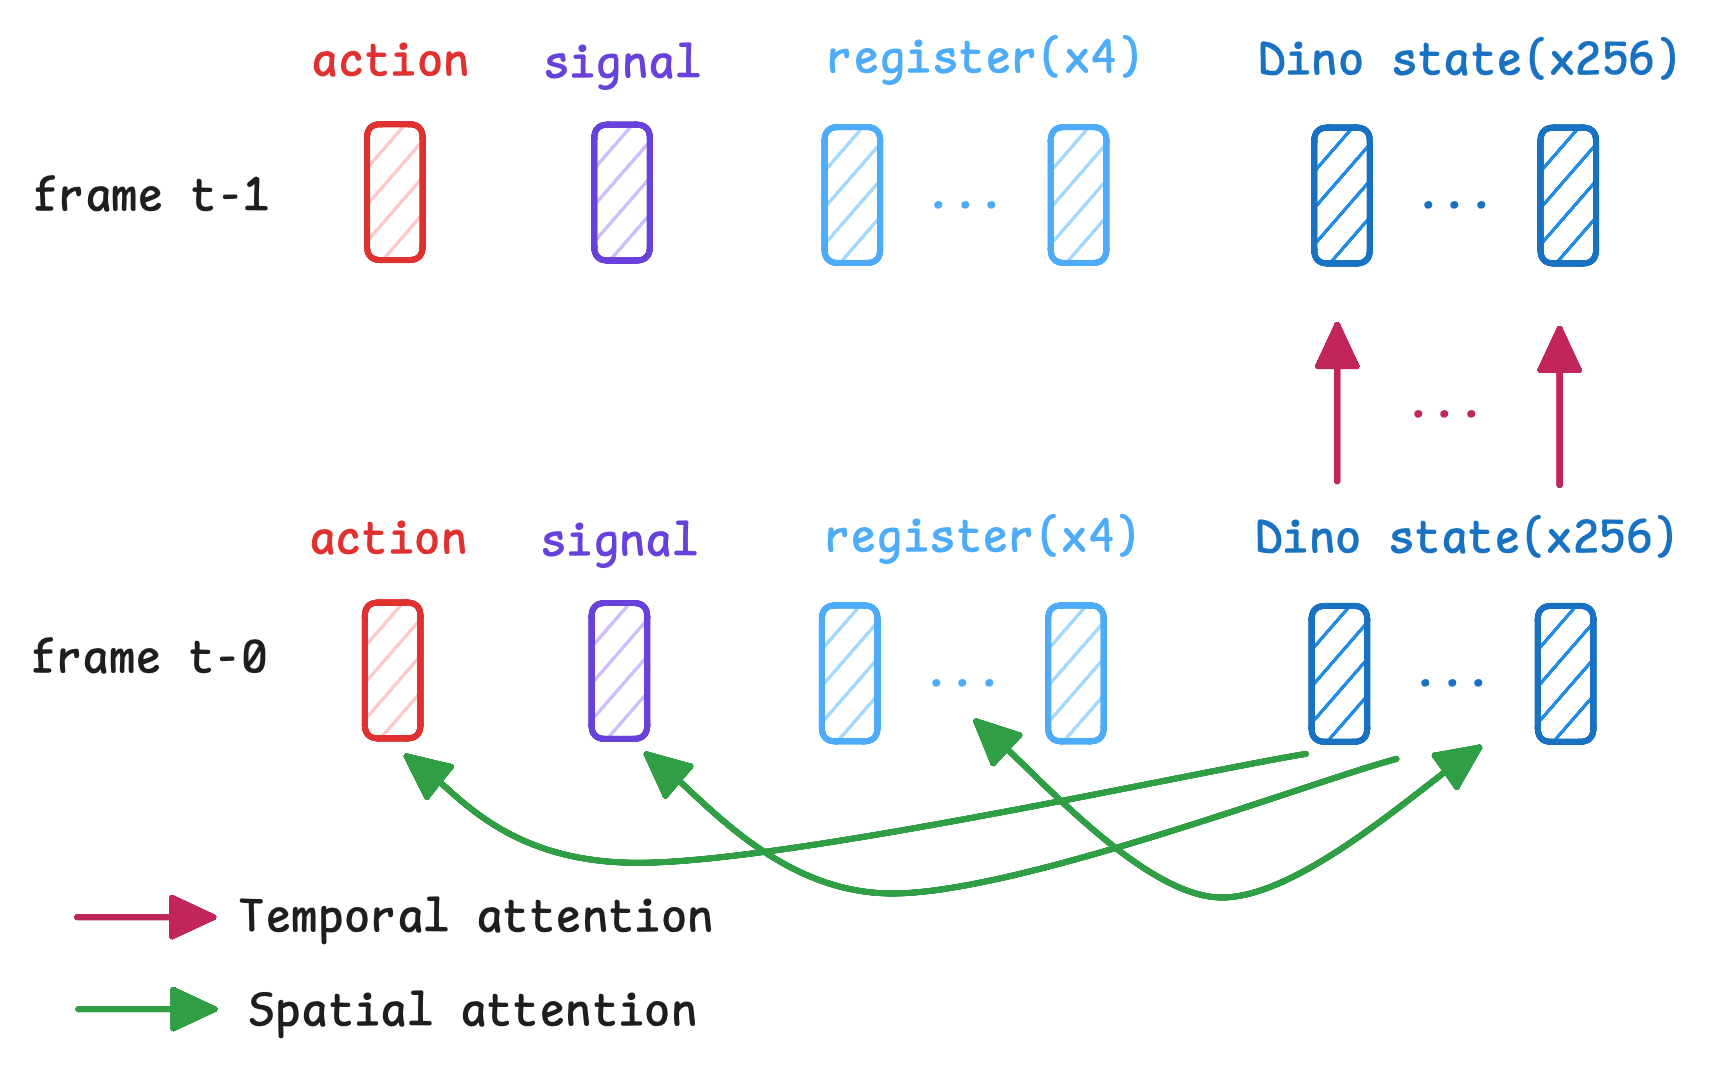
\includegraphics[width=0.6\textwidth]{images/token_layout_attention.png}
    \caption{Per-frame token layout and factorized attention. Spatial layers attend across signal, action, register, and patch tokens within the same frame. Temporal layers attend causally across time for each token position, allowing the model to propagate information through the sequence while preserving autoregressive rollout behavior.}
    \label{fig:token-layout-factorized-attention}
\end{figure}

The transformer alternates between two attention patterns. Most layers are spatial layers: they process each frame independently and allow all tokens inside the frame to attend to one another. Periodically, a temporal layer reshapes the sequence so that each token position attends along time with a causal mask. This factorization keeps the attention cost manageable while still allowing information to move both across image regions and across frames.

\subsection{Temporal Context and Independent Frames}
Temporal attention is causal and limited to a finite context window of the preceding 24 frames. Because all datasets are sampled at 5 Hz, this corresponds to 4.8 seconds of visual history rather than an arbitrary number of frame indices. Temporal layers are inserted every fourth transformer block, leaving three spatial blocks between consecutive temporal blocks. At rollout time, the same causal structure is used with a key-value cache. In transformer attention, each new query attends to keys and values computed from previous tokens; a KV cache stores those past keys and values so they can be reused instead of recomputed. When a new frame is generated, the model can therefore attend to the cached past without recomputing every previous transformer state. This is especially important for diffusion rollout, because each future frame requires many denoising steps. Without caching, planning would repeatedly pay the cost of re-encoding the same context for every candidate action sequence and every denoising iteration.

Following DreamerV4, training alternates between two prediction modes rather than treating every frame as a temporal transition \cite{hafner2025dreamerv4}. In the main run, each sampled frame is marked independent with probability 0.3; temporal attention for those frames is blocked, so they must be denoised from their own corrupted observation alone. Dependent frames, by contrast, may attend to earlier frames and use action information to infer how the scene evolves. The two cases therefore teach complementary behaviors: independent frames train single-frame denoising without relying on history, while dependent frames train the temporal dynamics needed for rollout. This prevents the model from solving every denoising task by leaning on nearby context and is useful in the mixed-data setting, where action-free videos should still contribute visual supervision even when no robot control is available. It is also compatible with diffusion forcing, because rollout conditions the model on generated rather than perfectly clean history. Future frames begin as noise, generated frames are fed back at an intermediate signal level, and passive video samples may not provide action information. Action supervision is applied only to dependent frames, because an independent frame has no meaningful transition context.

\section{Diffusion Forcing Objective}
\subsection{Signal-Level Corruption}
The model is trained with a Diffusion Forcing style objective \cite{chen2024diffusionforcing}. Instead of corrupting the whole sequence with one global diffusion time, each frame receives its own signal level $s_t \in [0,1]$. A signal level of 1 corresponds to a clean latent state and a signal level of 0 corresponds to pure Gaussian noise. For a clean latent $z_t$ and noise $\epsilon_t \sim \mathcal{N}(0,I)$, the corrupted latent is
\begin{equation}
\label{eq:signal-corruption}
x_t(s_t) = s_t z_t + (1-s_t)\epsilon_t .
\end{equation}
The signal levels are sampled independently across time, so a training sequence may contain clean context frames, moderately corrupted frames, and almost pure-noise future frames at the same time. The choice of training schedule is especially important here because the prediction target is a high-dimensional representation rather than a compact image code: one frame contains $256 \cdot 768 = 196{,}608$ scalar features. In such a space, a signal level that is appropriate for lower-dimensional latents can leave too much recoverable structure across the full feature vector, so training should spend more probability mass at lower signal levels. The RAE work addresses this with a dimension-aware resolution shift for high-dimensional representation latents \cite{dt_rae2025}, while Just Image Transformers motivates a logit-normal schedule when predicting clean data directly in high-dimensional representation spaces \cite{li2025jit}. The main model in this thesis uses the RAE-style resolution-shifted schedule, and Chapter 4 compares it against the JIT logit-normal schedule and a uniform baseline. Figure~\ref{fig:noise-schedule-distributions} shows the three distributions. The resolution-shifted schedule transforms a base uniform variable $u \in [0,1]$ according to
\begin{equation}
\label{eq:resolution-shifted-signal}
\begin{aligned}
s &= \frac{\alpha u}{1 + (\alpha - 1)u},
&
\alpha &= \sqrt{\frac{d_{\mathrm{base}}}{d_{\mathrm{eff}}}}.
\end{aligned}
\end{equation}
where $d_{\mathrm{base}}=4096$ and $d_{\mathrm{eff}}=256\cdot768$. Because the model is parameterized by signal level rather than noise time, this is the inverse form of the dimension-aware timestep shift used in RAE-style latent diffusion.

\begin{figure}[H]
    \centering
    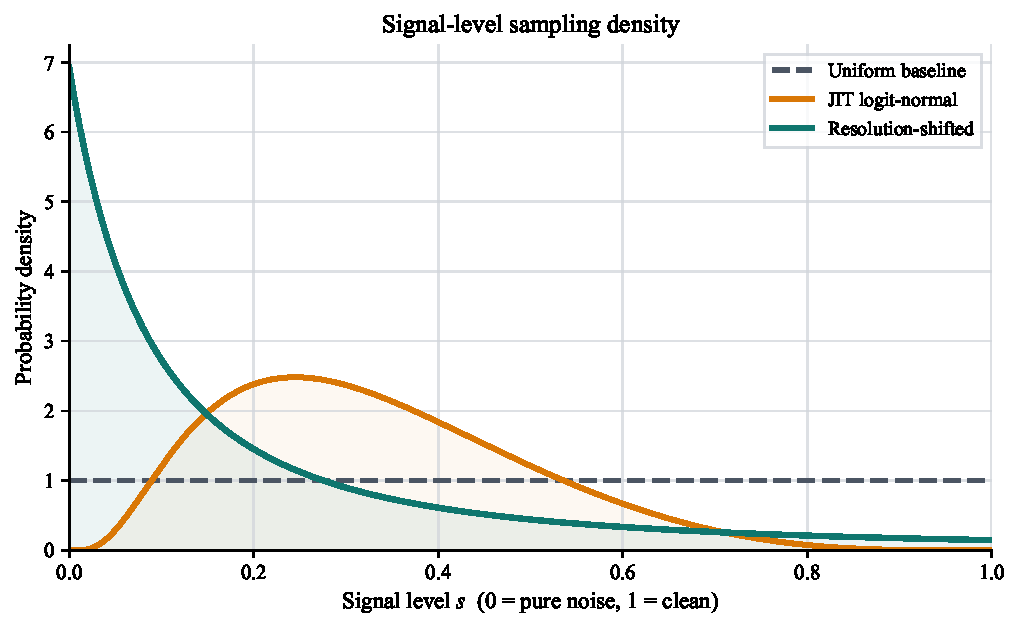
\includegraphics[width=0.78\textwidth]{images/noise_schedule_distributions.pdf}
    \caption{Distribution of signal levels sampled during training. The uniform baseline samples all signal levels equally. The JIT logit-normal schedule with $\mu=-0.8$ and $\sigma=0.8$ favors intermediate signal levels, corresponding to moderately corrupted latents. The resolution-shifted schedule used in the final model, with $\alpha=\sqrt{4096/196608}\approx0.144$, places more probability mass at low signal levels, so highly corrupted latents are sampled more often.}
    \label{fig:noise-schedule-distributions}
\end{figure}

\subsection{Endpoint Prediction and Velocity Loss}
Although the conceptual objective is flow matching, the network predicts a denoised endpoint $\hat{z}_t=f_\theta(x_{1:T},s_{1:T},a_{1:T})_t$. This means that the network is asked to estimate where the noisy latent should end up, rather than directly outputting the infinitesimal motion used by the sampler. The sampler still requires a velocity field, so the velocity is derived afterward from the direction between the current noisy state and the predicted clean endpoint. This choice is related to recent evidence from Just Image Transformers that direct clean-data prediction can be more robust than predicting noised quantities in very high-dimensional spaces \cite{li2025jit}. The velocity used by the solver is then derived from the straight interpolation path between the current noisy state and the predicted clean endpoint:
\begin{equation}
\label{eq:solver-velocity}
v_\theta(x_t,s_t) =
\frac{\hat{z}_t - x_t(s_t)}{\max(1-s_t,\delta)} ,
\end{equation}
where $\delta$ is a small denominator floor used for numerical stability. For the same interpolation path, the target velocity is
\begin{equation}
\label{eq:target-velocity}
v^\star_t = z_t - \epsilon_t .
\end{equation}
The training loss used in the main runs is the mean squared error between predicted and target velocity,
\begin{equation}
\label{eq:velocity-loss}
\mathcal{L}_{\mathrm{vel}} =
\mathbb{E}\left[
\frac{1}{|\Omega|}
\sum_{t \in \Omega}
\left\|v_\theta(x_t,s_t)-v^\star_t\right\|_2^2
\right],
\end{equation}
where $\Omega$ is the set of valid, non-padded frames in the batch. Fixed-length sequence sampling can request frames beyond the end of an episode, in which case the dataset returns repeated terminal frames together with a padding mask. These repeated frames do not correspond to real future transitions, so they are excluded from the loss. The loss is computed over all DINO patch tokens and feature dimensions. The logger also reports loss separately for independent frames, dependent frames, action-conditioned frames, and action-free frames, which makes it possible to detect whether the model is only learning static denoising or is also learning temporally and action-conditioned prediction.

\subsection{Sampling and Latent Rollout}
At inference time, rollout begins from the observed context frames. These frames are encoded with the frozen DINOv2 encoder and processed once by the spatial-temporal transformer at signal level 1. Their attention keys and values are stored in a key-value (KV) cache, so later predictions can attend to the already processed history without recomputing the full context at every denoising step.

Each future frame is then generated autoregressively. A new latent state is initialized from Gaussian noise, combined with register tokens, its current signal level, and the action for that time step, and passed through the transformer while attending to the cached history. The Euler solver repeatedly queries the same model as the signal level increases from noise toward a clean latent state. For a sequence of solver times $0=s_0 < s_1 < \cdots < s_K=1$, the update is
\begin{equation}
\label{eq:euler-update}
x_{k+1}=x_k + v_\theta(x_k,s_k)(s_{k+1}-s_k).
\end{equation}
The number of solver steps controls the trade-off between denoising accuracy and rollout cost. Once a future latent has been generated, it becomes part of the history for the next prediction. Instead of inserting it into the cache as perfectly clean context, the latent is re-noised to a fixed non-clean rollout signal level before it is processed once more and appended to the KV cache. This is where Diffusion Forcing enters the rollout procedure: the model is trained on mixed-noise sequences and is therefore asked during rollout to condition on generated history that is also non-clean. Figure~\ref{fig:latent-rollout-kv-cache} summarizes this loop, which combines iterative denoising for the current frame with efficient cached conditioning on all previously observed and generated frames.

\begin{figure}[H]
    \centering
    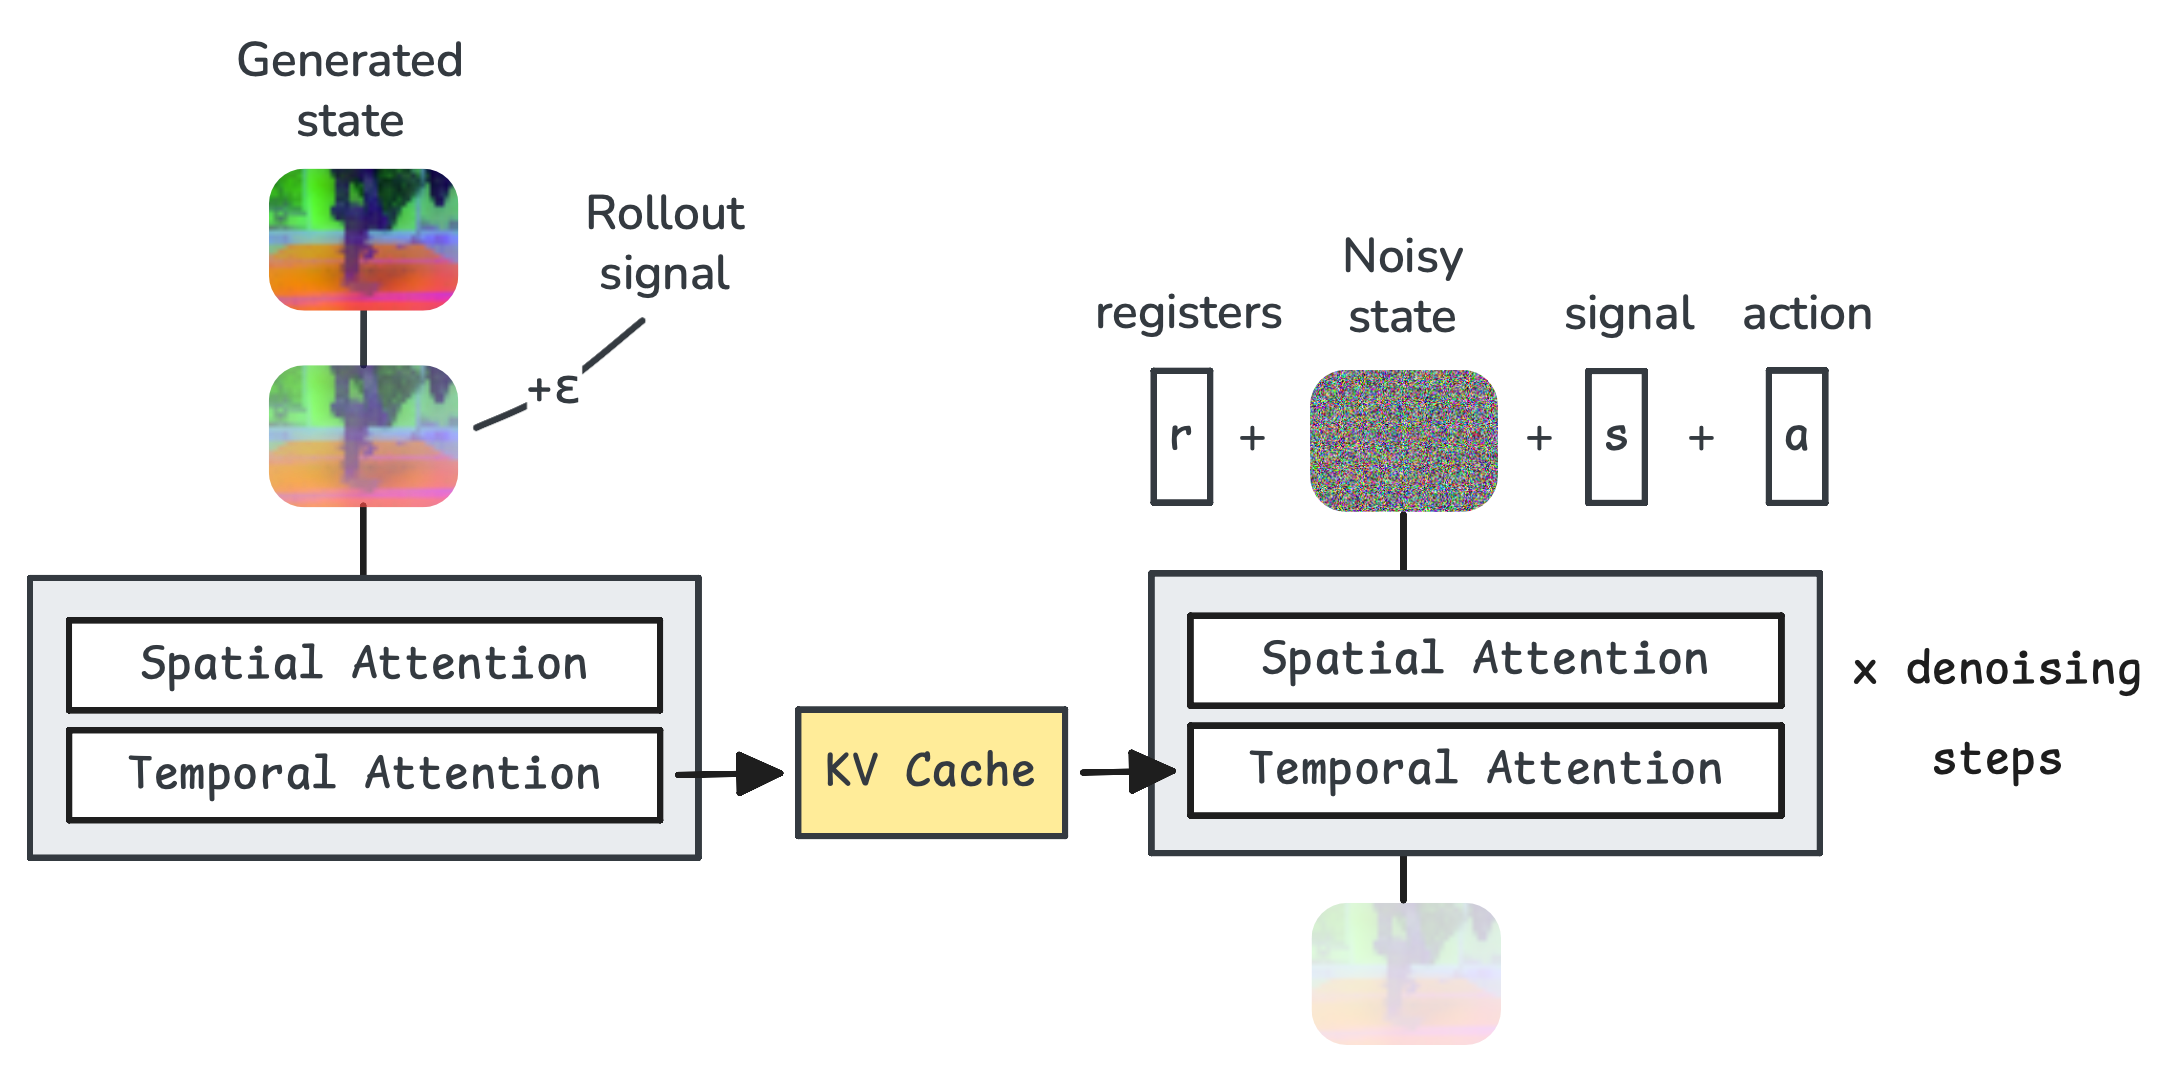
\includegraphics[width=0.8\textwidth]{images/rollout_with_kv_cache.png}
    \caption{Autoregressive latent rollout with Diffusion Forcing, KV caching, and Euler denoising. Observed and previously generated states are processed once and stored in the KV cache. To generate the next state, a noisy latent is denoised over multiple Euler steps while attending to this cached history together with the current signal level and action. After generation, the new latent is fed back at a fixed non-clean rollout signal before being added to the cache for subsequent predictions.}
    \label{fig:latent-rollout-kv-cache}
\end{figure}

\section{Dataset Pipeline}
\subsection{UR5 Data Recording}
The UR5 dataset used in this thesis was recorded with an extension of LeRobot, an open-source PyTorch framework for real-world robot learning that provides tools for recording, storing, and loading robot datasets \cite{cadene2024lerobot}. UR5 support was added through the RTDE control interface, which made it possible to use the existing LeRobot recording pipeline while teleoperating the robot with a smartphone interface.

The goal of the recording was not to collect goal-directed imitation-learning demonstrations. Instead, the dataset was designed to contain broad interaction dynamics. A set of 10 tabletop objects was used, and approximately two hours of data were recorded by teleoperating the robot while interacting with the objects without a fixed task goal: picking them up, dropping them, stacking them, moving them, and creating varied contact situations. This is deliberately different from a task-oriented imitation dataset, where each episode is usually recorded to solve a specific goal. Here, the objective was to cover a wide range of robot motions and object interactions so that the world model could learn visual dynamics rather than imitate a narrow policy. A single camera was used at a time, but its position was changed between episodes so that the robot was seen from varied viewpoints rather than from one fixed laboratory angle.

The raw recordings contain images, end-effector state, gripper state, and robot timing information. After recording, the trajectories are converted to 5 Hz action sequences. The action target is not the raw teleoperation command, but the future end-effector pose reached after one 5 Hz step.
Let $(p_t,R_t,g_t)$ denote the current end-effector position, orientation, and gripper state, and let $(p_{t+1},R_{t+1},g_{t+1})$ denote the next 5 Hz target pose. The action representation is defined in the local end-effector frame as
\begin{equation}
\label{eq:ur5-action-deltas}
\begin{aligned}
\Delta p_{\mathrm{local}} &= R_t^{-1}(p_{t+1}-p_t),\\
\Delta R_{\mathrm{local}} &= R_t^{-1}R_{t+1},\\
\Delta g &= g_{t+1}-g_t .
\end{aligned}
\end{equation}
The translational displacement is expressed in the current end-effector frame, so the same token describes motion relative to the tool rather than relative to the fixed robot base. For orientation, the relative rotation $\Delta R_{\mathrm{local}}$ is computed first and then stored as a rotation vector. The two absolute rotation vectors are not subtracted directly, because rotation vectors are a coordinate representation of orientation rather than positions in a globally linear space. Computing the relative rotation first gives the actual rotational displacement between the two end-effector poses. Finally, the resulting translation, orientation, and gripper deltas are normalized with dataset statistics before they are used as action tokens.

\subsection{Common LeRobot Format}
All training sources are accessed through a common LeRobot-style dataset interface. Each dataset specification provides its repository, available cameras, action mode, target frame rate, and sequence length. Training uses sequences of 32 frames at 5 Hz, so each training example spans 6.4 seconds. For each sample, one camera stream is selected according to configured camera weights, a fixed-length sequence is loaded at the target frame rate, frames are resized and center-cropped to $224 \times 224$, and actions are converted to the requested token representation when they exist. If the requested sequence extends beyond the end of an episode, the dataset supplies padded frames and a validity mask so that these artificial frames can be ignored by the loss.

Dataset balancing is done through a virtual mixture rather than by physically merging the datasets. This balancing is based on duration rather than raw frame count. A naive frame-indexed mixture would over-represent datasets stored at higher native frame rates, even if they contain the same amount of real time. To avoid this, each dataset is converted to an effective length at the target 5 Hz sampling rate, and the virtual index map is built so that the configured weights correspond to proportions of real interaction time. This makes the mixture explicit and reproducible while still allowing very different datasets to be sampled in a single distributed dataloader.

\subsection{Mixed Video and Robot Training}
The main training recipe is a single mixed-data regime rather than a strict pretraining-then-fine-tuning pipeline. This choice was made because the action interface is part of the transformer input: pretraining an action-free model and adding a new action pathway only during fine-tuning changes the input distribution and can be destructive. Preliminary experiments in this project found the mixed regime to be more robust and to give better held-out performance than adding action conditioning after pretraining. The action-capable model is therefore trained on both action-labeled UR5 data and action-free video data from the start. This is possible because action availability is represented by whether a projected action embedding is added to the base action token: UR5 samples can condition on real controls, while BridgeData V2, EPIC-KITCHENS, and DROID samples still contribute visual dynamics without requiring compatible actions \cite{walke2023bridgedatav2,damen2022epickitchens,khazatsky2024droid}.

The datasets were chosen to emphasize interaction-heavy video without making storage the dominant constraint. The UR5 data provides the target robot embodiment and the only action-labeled supervision used for control. BridgeData V2 adds robot manipulation videos from a different robot setup. DROID adds more diverse in-the-wild robot manipulation scenes. EPIC-KITCHENS contributes egocentric human-object interaction, which is not robotic but contains many contact-rich visual changes that are useful for learning general video dynamics.

The training mixture is summarized in Table~\ref{tab:training-mixture}. All sources are sampled at 5 Hz. UR5 contributes 25\% of the sampled training time and provides the action-labeled robot transitions. Following DreamerV4, projected action embeddings on dependent UR5 frames are masked with probability 0.3, leaving only the learned base action token \cite{hafner2025dreamerv4}. This keeps an unconditioned denoising pathway active even on action-labeled data, so the model learns from both controlled trajectories and unconditioned videos instead of relying only on action-conditioned denoising. The remaining datasets are loaded with no action mode, so no projected action embedding is added. This gives the model two kinds of supervision at once: broad visual prediction from heterogeneous videos and action-conditioned dynamics from the robot domain.

\begin{table}[H]
\caption{Mixed training dataset. All datasets are converted to the same latent sequence format. UR5 data supplies action-conditioned transitions, while the remaining datasets train visual dynamics through the masked action-token path.}
\label{tab:training-mixture}
\begin{center}
\small
\begin{tabular}{@{}l c c L{0.44\textwidth}@{}}
\toprule
\textbf{Dataset source} & \textbf{Weight} & \textbf{Actions} & \textbf{Role in training} \\
\midrule
UR5 recordings & 0.25 & yes & Target robot embodiment, varied camera positions, and action-conditioned transitions. \\
BridgeData V2 & 0.15 & no & Additional robot manipulation video from a different setup. \\
EPIC-KITCHENS & 0.30 & no & Egocentric human-object interaction and non-robot visual dynamics. \\
DROID & 0.30 & no & In-the-wild robot manipulation video diversity. \\
\bottomrule
\end{tabular}
\end{center}
\end{table}

\subsection{Optimization}
Training is performed with distributed data parallelism, bfloat16 autocast, AdamW, and gradient clipping at norm 1.0. The final model contains approximately 400 million trainable parameters and the main experiments were trained on four NVIDIA H200 GPUs on the University of Tartu UT Rocket high-performance computing cluster \cite{utrocket2018}. The mixed corpus used in the experiments contains roughly 1{,}000 hours of video after dataset selection and temporal resampling. Each dataloader batch contains 128 sequences of 32 frames, corresponding to 4{,}096 sampled frames before padded frames are removed. Gradient accumulation over four minibatches is used to obtain a larger effective batch while keeping the memory footprint of each forward and backward pass within GPU memory limits. The learning rate is warmed from $10^{-7}$ to $3\cdot10^{-4}$ during the first 500 optimizer steps. The loss is normalized by the number of valid frames across all distributed workers, rather than by the local batch size, so that partially padded sequences do not change the effective scale of the update. Checkpoints are saved periodically and can be loaded strictly when resuming the same run or non-strictly when initializing compatible variants of the model.

\section{Evaluation Protocol}
Evaluation measures two related properties of the learned dynamics. The first is local conditional prediction: given a real context frame and the action for the next transition, can the model denoise the next latent state? The second is autoregressive rollout quality: after observing a short context, how far does the generated trajectory drift from the real future when its own predictions are fed back into the temporal cache?

The evaluation loader uses a held-out UR5 dataset with one camera view and teleoperated episodes sampled at 5 Hz. It loads 85-frame sequences, and rollout evaluation begins after the first 10 frames, giving the model 2 seconds of observed context before future prediction is measured. Evaluation is action-conditioned. The robot control is a 7-dimensional end-effector delta, consisting of translation, rotation-vector orientation, and gripper change. Padded frames are excluded by the validity mask, so metrics are accumulated only over real transitions.

For the teacher-forced metric, every valid adjacent pair $(z_t,z_{t+1})$ is treated as a one-step prediction problem. The model first processes $z_t$ as clean context at signal level 1, then samples $z_{t+1}$ from noise using the Euler solver and the ground-truth action token. The final prediction is compared to the target latent with mean squared error over all patch tokens and feature dimensions. The normalization factor $256\cdot768$ comes from the DINO representation defined in Equation~\ref{eq:dino-latent-shape}: each frame contains 256 patch tokens, and each token has 768 feature dimensions,
\begin{equation}
\label{eq:teacher-forced-mse}
\mathcal{E}_{\mathrm{TF}} =
\frac{1}{|\mathcal{V}|}
\sum_{(t,t+1)\in\mathcal{V}}
\frac{1}{256\cdot768}
\left\|
\hat{z}_{t+1}-z_{t+1}
\right\|_2^2 ,
\end{equation}
where $\mathcal{V}$ is the set of valid, non-padded transitions.

For rollout evaluation, the first observed frames are encoded as context and the remaining frames are generated autoregressively with the ground-truth action sequence. After each generated future frame, the prediction is re-noised to the configured rollout signal level before being inserted into the cache for the next step. This matches the Diffusion Forcing rollout procedure described above and avoids evaluating the model only under clean teacher-forced history. The evaluator reports MSE at several rollout horizons using the same per-frame DINO-latent normalization,
\begin{equation}
\label{eq:rollout-mse}
\mathcal{E}_{H} =
\frac{1}{|\mathcal{B}_H|H}
\sum_{b\in\mathcal{B}_H}
\sum_{h=1}^{H}
\frac{1}{256\cdot768}
\left\|
\hat{z}_{b,t+h}-z_{b,t+h}
\right\|_2^2 ,
\end{equation}
where $\mathcal{B}_H$ contains sequences for which the context and all $H$ future frames are valid. Reporting several horizons is more informative than a single average, because short-horizon errors mostly measure local dynamics while longer horizons expose compounding rollout drift.

The evaluator also logs qualitative videos for selected samples. It decodes the ground-truth latent sequence and the action-conditioned rollout using the RAE decoder. These videos are not used to compute the metrics, but they make it possible to interpret the latent errors in terms of visible scene consistency, object motion, and loss of task-relevant structure.

\section{Planning with the World Model}
\subsection{Goal-Conditioned Latent Cost}
Planning is formulated as goal-conditioned trajectory optimization in the frozen DINO feature space. Given a current image $I_t$ and a goal image $I_g$, both are encoded into latent states $z_t$ and $z_g$. A candidate future action sequence $\mathbf{a}_{t:t+H-1}$ is converted into action tokens and rolled out through the world model to produce $\hat{z}_{t+1:t+H}$. The primary objective is terminal latent distance with a small action penalty,
\begin{equation}
\label{eq:planning-objective}
J(\mathbf{a}_{t:t+H-1}) =
\frac{1}{256\cdot768}
\left\|
\hat{z}_{t+H} - z_g
\right\|_2^2
+
\lambda
\frac{1}{H}
\sum_{h=0}^{H-1}
\| \Delta a_{t+h} \|_2^2 .
\end{equation}
The latent term measures whether the imagined final observation resembles the goal in the DINO feature space. The action term discourages unnecessarily large end-effector moves and encourages the optimizer to distribute motion more evenly over the horizon instead of solving the task with a small number of abrupt jumps. The coefficient $\lambda$ controls the trade-off between terminal latent distance and the action penalty, and is set to $0.2$.

\subsection{Cross-Entropy Method}
The action sequence is optimized with the Cross-Entropy Method (CEM) \cite{botev2013cem}. CEM is a derivative-free optimizer that repeatedly samples candidate solutions, keeps the best samples, and refits its sampling distribution around those elites. In this setting, the distribution is a diagonal Gaussian over denormalized end-effector delta sequences. At each iteration, a population of candidate action sequences is sampled, each dimension is clamped to a physically reasonable range, the candidates are converted into normalized action tokens, and the world model rolls them out in latent space. The candidates are then scored by the cost above, and the mean and variance of the Gaussian are updated from the elite subset. The zero-action sequence and the current mean are also evaluated as candidates, which gives the optimizer stable baselines during early iterations.

The decoder is not part of the planner. CEM only sees latent costs computed in DINO feature space. After optimization, the RAE decoder can be used to visualize selected imagined rollouts for debugging: for example, to check whether a low latent cost corresponds to plausible object motion or whether the model has found an unrealistic latent-space shortcut. These decoded videos are qualitative diagnostics only and do not affect the selected action sequence.

%%==========================================================================
%% CHAPTER 4: EXPERIMENTS AND RESULTS
%%==========================================================================
\chapter{Experiments and Results}

\section{World Model Prediction Quality}
This section first studies the main training and rollout choices that determine the final world-model configuration, then inspects the resulting model qualitatively. All quantitative comparisons follow the held-out UR5 evaluation protocol described in Chapter 3 and report mean squared error in DINO-latent space, averaged over patch tokens and feature dimensions. The teacher-forced metric measures one-step conditional prediction: the model is given a clean real latent frame and the ground-truth action, then its generated next latent is compared with the real next latent. The rollout metrics measure autoregressive prediction: after ten clean context frames, the model receives only the ground-truth future actions, feeds its own generated latents back into the temporal cache, and is compared with the real evaluation trajectory at horizons $H=5$, $H=10$, and $H=20$. Lower values are better for all reported metrics.

The experiments use roughly 1{,}000 hours of selected video, a 400-million-parameter model, and four NVIDIA H200 GPUs. This remains modest relative to contemporary generative video work: Wan reports 1.3-billion- and 14-billion-parameter variants trained on billions of images and videos, while Dreamer 4 uses a 1.6-billion-parameter dynamics model inside a 2-billion-parameter world-model system \cite{wan2025wan,hafner2025dreamerv4}. The purpose of the experiments below is therefore to characterize the behavior of the proposed design under a bounded compute budget, not to claim parity with larger video foundation models.

\subsection{Effect of Mixed-Data Training}
The first comparison studies how much the target UR5 data benefits from being mixed with broader video sources. Four runs are compared: a UR5-only model and mixtures where UR5 contributes 50\%, 25\%, or 10\% of the sampled training time. Each run was continued until the held-out evaluation metrics no longer improved, and Table~\ref{tab:dataset-mixture-results} reports the best evaluation checkpoint from that run rather than forcing all models to be compared at the same training step. A same-step comparison would answer a different question, because one expected benefit of adding more diverse data is precisely that it delays overfitting and permits useful training to continue for longer. Figure~\ref{fig:chart-mix-data} visualizes the same trade-off across rollout horizons.

\begin{figure}[H]
    \centering
    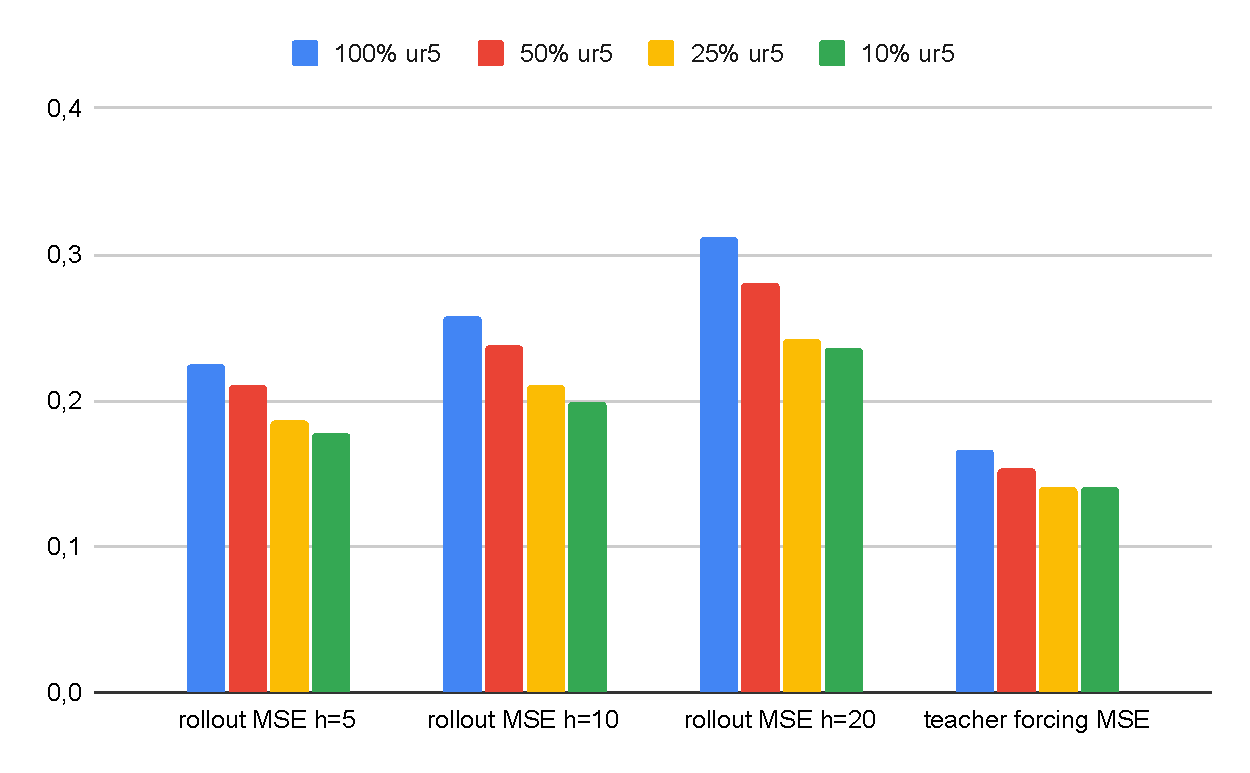
\includegraphics[width=0.82\textwidth]{images/chart_mix_data.pdf}
    \caption{Held-out UR5 prediction error for different data mixtures. Increasing the amount of mixed video data improves rollout quality, but the gains become small when moving from the 25\% UR5 mixture to the 10\% UR5 mixture.}
    \label{fig:chart-mix-data}
\end{figure}

\begin{table}[h]
\caption{Effect of mixed-data training on held-out UR5 prediction using the evaluation protocol of Chapter 3. Each row reports the best evaluation checkpoint reached before the corresponding run stopped improving. The mixed-video configurations use UR5 together with BridgeData V2 \cite{walke2023bridgedatav2}, EPIC-KITCHENS \cite{damen2022epickitchens}, and DROID \cite{khazatsky2024droid}. Metrics are DINO-latent mean squared errors; lower is better, and the best metric in each error column is shown in bold.}
\label{tab:dataset-mixture-results}
\begin{center}
\small
\begin{tabular}{@{}L{0.26\textwidth} c c c c c@{}}
\toprule
\textbf{Training mixture} & \textbf{Best} & \textbf{Teacher-Forcing} & \multicolumn{3}{c}{\textbf{Rollout MSE}} \\
\cmidrule(lr){4-6}
 & \textbf{Step} & \textbf{MSE} & \textbf{$H=5$} & \textbf{$H=10$} & \textbf{$H=20$} \\
\midrule
UR5 only & 2{,}000 & 0.166 & 0.224 & 0.257 & 0.312 \\
50\% UR5, 50\% mixed & 5{,}500 & 0.153 & 0.210 & 0.238 & 0.280 \\
25\% UR5, 75\% mixed & 15{,}500 & \textbf{0.141} & 0.186 & 0.210 & 0.242 \\
10\% UR5, 90\% mixed & 35{,}500 & 0.148 & \textbf{0.178} & \textbf{0.199} & \textbf{0.236} \\
\bottomrule
\end{tabular}
\end{center}
\end{table}

The UR5-only run began to overfit quickly, as expected from the limited size of the target-domain dataset, and its best held-out checkpoint was reached after only 2{,}000 optimizer steps. Adding external video data allowed useful training to continue for much longer: the 50\% UR5 mixture improved until 5{,}500 steps, the 25\% UR5 mixture until 15{,}500 steps, and the 10\% UR5 mixture only reached its best evaluation point after 35{,}500 steps. This confirms that mixed video delays overfitting and improves rollout stability.

However, the improvement from 25\% to 10\% UR5 is small compared with the additional training time. The 10\% mixture gives the lowest rollout errors at horizons 5, 10, and 20, but it slightly worsens the teacher-forced metric and requires more than twice as many optimizer steps as the 25\% mixture. This suggests a practical plateau for the present model size and compute budget: after enough mixed video has been added, further reducing the amount of target-robot data mostly increases the time needed to reach the best checkpoint. For this reason, the remaining ablations use the 25\% UR5 mixture, which provides nearly the same rollout quality with faster experimental iteration.

\subsection{Effect of Training Noise Schedule}
The signal-level distribution is a training choice. Chapter 3 introduced a resolution-shifted schedule because the DINO latent state is much higher-dimensional than a conventional compressed VAE latent. This recommendation follows the RAE work on high-dimensional representation latents \cite{dt_rae2025}. At the same time, Just Image Transformers reports strong results from a logit-normal schedule when predicting clean data in high-dimensional representation spaces \cite{li2025jit}. It is therefore useful to compare both schedules directly in the present world-model setting, together with a uniform baseline. The final 25\% UR5 mixed-data setting is used for this ablation, and Table~\ref{tab:noise-schedule-results} reports the best held-out UR5 checkpoint for each run.

\begin{table}[h]
\caption{Effect of the training signal-level sampling schedule on held-out UR5 prediction in the 25\% UR5 mixed-data setting. Metrics are DINO-latent mean squared errors; lower is better.}
\label{tab:noise-schedule-results}
\begin{center}
\small
\begin{tabular}{@{}l c c c c c@{}}
\toprule
\textbf{Signal schedule} & \textbf{Best} & \textbf{TF} & \multicolumn{3}{c}{\textbf{Rollout MSE}} \\
\cmidrule(lr){4-6}
 & \textbf{step} & \textbf{MSE} & \textbf{$H=5$} & \textbf{$H=10$} & \textbf{$H=20$} \\
\midrule
Uniform & 15{,}500 & 0.142 & 0.213 & 0.245 & 0.283 \\
Logit-normal & 16{,}000 & \textbf{0.141} & 0.205 & 0.232 & 0.263 \\
Resolution-shifted & 15{,}500 & \textbf{0.141} & \textbf{0.186} & \textbf{0.210} & \textbf{0.242} \\
\bottomrule
\end{tabular}
\end{center}
\end{table}

The logit-normal and resolution-shifted schedules reach the same teacher-forced error, indicating similar local one-step denoising quality. The difference appears once predictions are fed back autoregressively: the resolution-shifted schedule lowers rollout error at every reported horizon, with the gap increasing from $H=5$ to $H=20$. The uniform baseline is clearly worse at the longest reported horizon, reaching $0.283$ at $H=20$ compared with $0.263$ for the logit-normal schedule and $0.242$ for the resolution-shifted schedule. This quantitative degradation also appeared qualitatively in decoded rollouts, where the uniform-schedule model tended to drift in later rollout steps, around 50 generated frames. These results confirm that adapting the training distribution over signal levels matters in this high-dimensional latent space.

\subsection{Rollout Feedback Signal Level}
The feedback signal level is an evaluation-time rollout choice. The learned denoiser is reused many times during autoregressive rollout, so long-horizon quality depends not only on the trained weights but also on how generated latent states are fed back into the temporal cache. After each future latent is generated, it is re-noised before being used as context for the next prediction. If the feedback state is too clean, evaluation becomes closer to teacher forcing than to the mixed-noise contexts seen during training; if it is too noisy, useful temporal information is unnecessarily destroyed.

The appropriate feedback level is especially worth revisiting in this thesis because the state representation differs strongly from the compact VAE latents commonly used in latent diffusion systems. For a compact latent state, even a small amount of added noise can remove a meaningful fraction of the available information, so feeding back nearly clean generated states is a reasonable default. Here, one frame contains $256\cdot768$ DINO features. As discussed in Chapter 3, the same scalar signal level does not imply the same effective corruption when the latent dimensionality changes by orders of magnitude. A feedback level that would be unnecessarily destructive in a low-dimensional VAE space may still leave a high-dimensional semantic state relatively informative. The sweep therefore tests a broad range of signal levels, from strongly noised feedback at $0.2$ to perfectly clean feedback at $1.0$, in order to identify how much generated-history corruption is useful for this representation space. Figure~\ref{fig:rollout-feedback-signal-level} reports this sweep.

\begin{figure}[H]
    \centering
    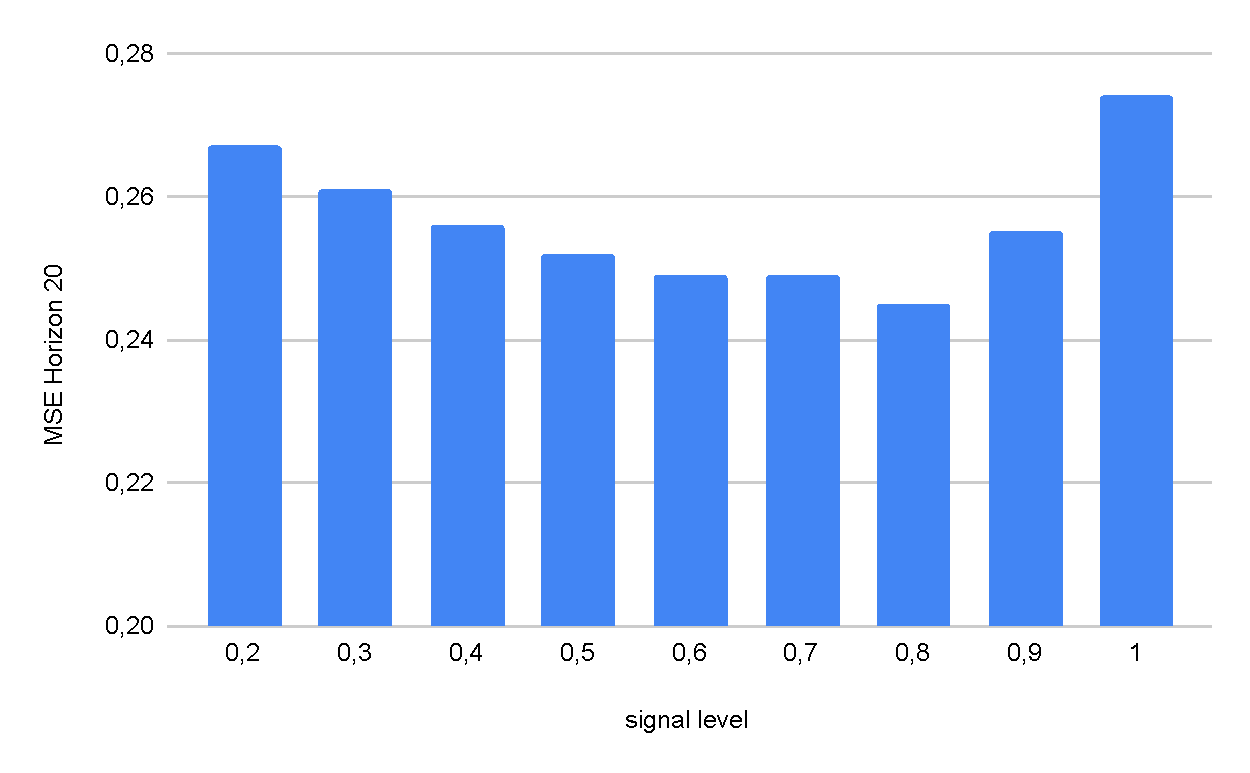
\includegraphics[width=0.72\textwidth]{images/rollout_feedback_signal_level.pdf}
    \caption{Effect of rollout feedback signal level on held-out UR5 rollout quality at horizon $H=20$. Lower signal levels correspond to stronger corruption before generated frames are fed back into the temporal cache. Intermediate feedback levels perform best, with the lowest error near $0.8$, while both strongly corrupted feedback and perfectly clean feedback degrade long-horizon rollout quality.}
    \label{fig:rollout-feedback-signal-level}
\end{figure}

The sweep shows that neither extreme is optimal for this representation space. Feeding generated history back at signal level $0.8$ gives the lowest $H=20$ rollout error, while both heavier corruption and perfectly clean feedback increase the error. This supports the use of partially corrupted generated context during rollout, rather than treating clean feedback as the default.

\subsection{Qualitative Rollouts}
The ablations above lead to the configuration used for the qualitative rollout examples. Figure~\ref{fig:result-world-model-rollouts} shows one representative action-conditioned rollout from a held-out UR5 evaluation episode. The model receives ten clean context frames from the episode, after which it is given only the ground-truth action sequence and must generate the future latent trajectory autoregressively. The sequence is displayed from frame 10 onward: the first image shown is the final clean context frame, while the remaining images compare the decoded generated latents with the corresponding evaluation frames. The rollout itself is produced at the normal 5 Hz evaluation rate, but the visualization displays one frame per second so that larger changes can be shown compactly. The decoder is used only for visualization; neither training nor quantitative evaluation uses reconstructed RGB images.

\begin{figure}[H]
    \centering
    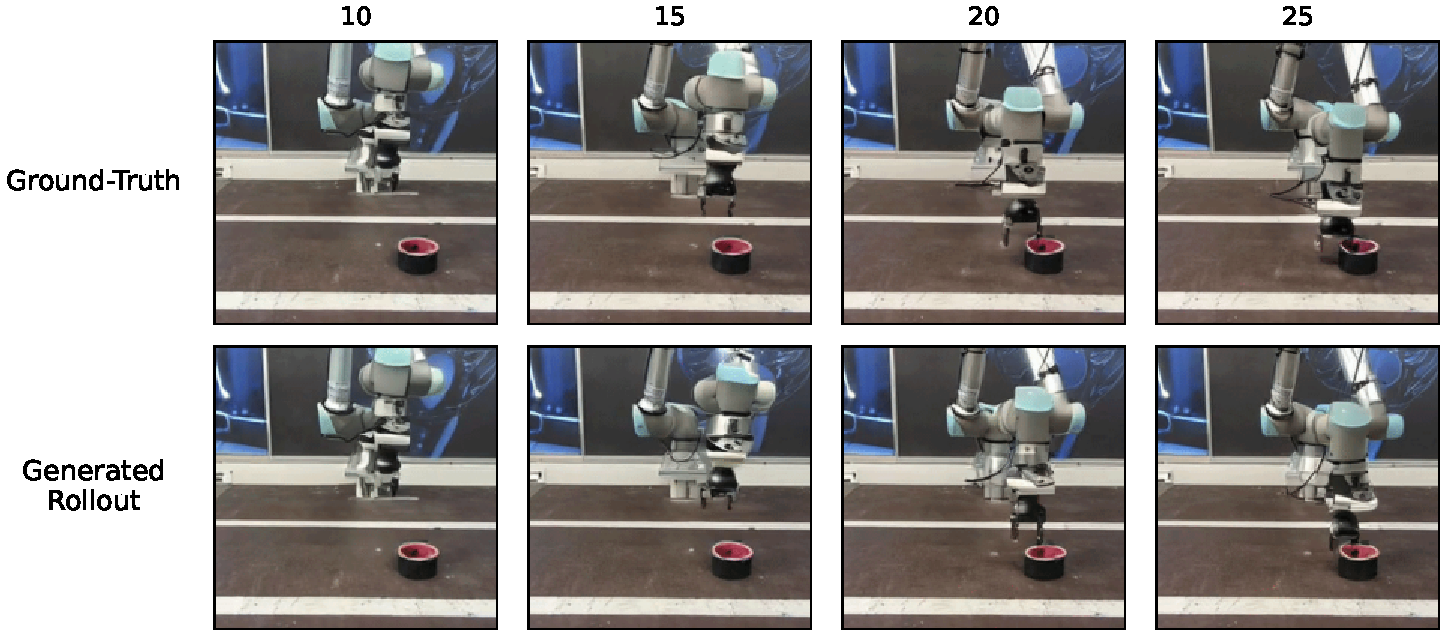
\includegraphics[width=1.0\textwidth]{images/comparison_0_part1.pdf}
    \\[2mm]
    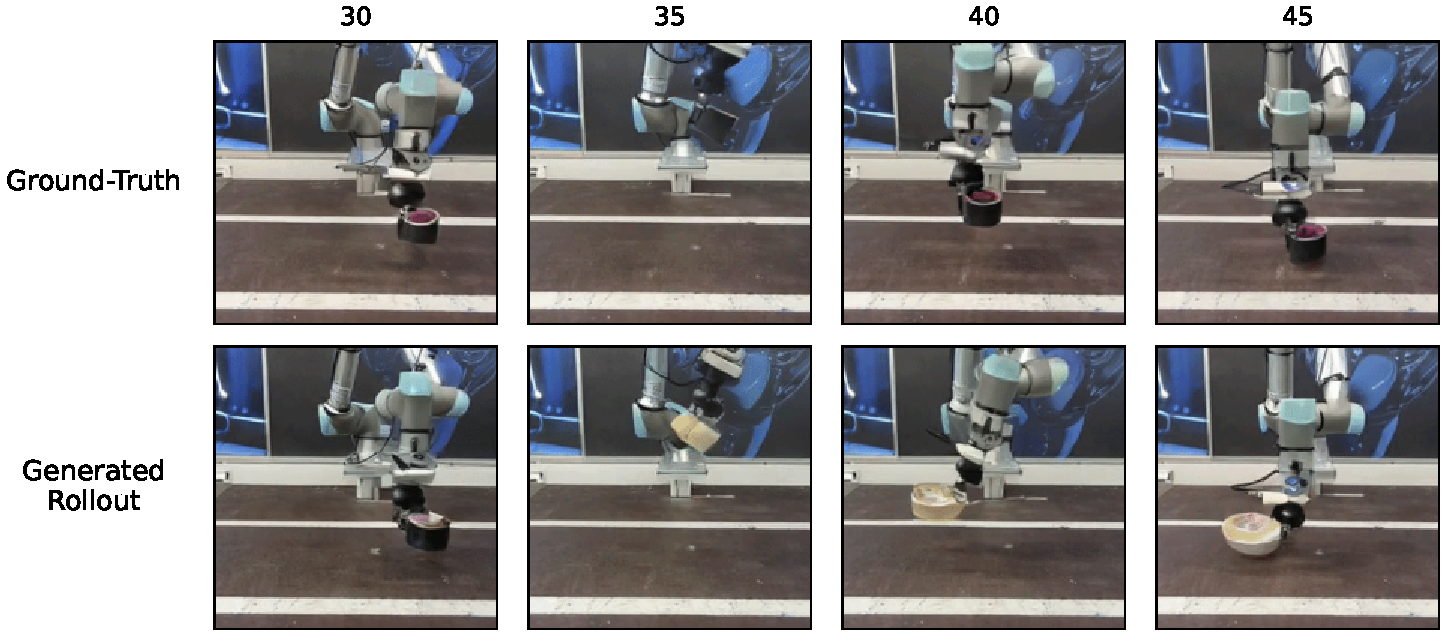
\includegraphics[width=1.0\textwidth]{images/comparison_0_part2.pdf}
    \caption{Qualitative world-model rollout on a held-out UR5 sequence. The upper row in each panel shows the ground-truth future and the lower row shows the decoded model rollout generated under the same ground-truth action sequence. Frame 10 is the final clean context frame after the 10-frame observation prefix; subsequent displayed frames are sampled every five frames, corresponding to one displayed frame per second from the 5 Hz rollout.}
    \label{fig:result-world-model-rollouts}
\end{figure}

Qualitatively, the generated sequence does not visibly drift away from the scene over the shown horizon: the background remains stable and the robot motion closely follows the ground-truth trajectory under the provided actions. The main limitation appears during object interaction in the later part of the rollout. The model continues to predict the robot motion accurately, but it fails to preserve the manipulated object's identity, with the object changing appearance while suspended in the gripper. This suggests that the learned dynamics capture robot kinematics more reliably than object-level interaction dynamics, especially when contact, occlusion, and larger 5 Hz action steps create substantial visual changes between consecutive frames. Additional qualitative rollout examples are provided in Appendix~\ref{app:additional-rollouts}.

\section{Offline Planning Diagnostics}
\subsection{DINO Distance as a Planning Cost}
The planner will select actions by minimizing a latent distance to a goal observation, so it is useful to first inspect whether this distance behaves like a meaningful progress signal. Before DINO feature distance is used as the planning cost, it is compared with raw pixel mean squared error on a held-out UR5 sequence. For this diagnostic, the last frame of a short episode is used as the goal frame. Each earlier frame is compared to this final frame, producing a distance-to-goal curve over time. The distance is computed both in normalized pixel space and in DINOv2 patch-feature space. To test robustness to nuisance visual changes, perturbed versions of the same video are also created by applying random brightness and contrast changes; the shaded areas in Figure~\ref{fig:goal-distance-comparison} show the variation induced by these perturbations.

\begin{figure}[H]
    \centering
    \resultfigure{1.0\textwidth}{images/results_goal_distance_timeline.png}
    \\[2mm]
    \resultfigure{1.0\textwidth}{images/distance_comparison_plot.png}
    \caption{Goal-distance diagnostic on a held-out UR5 evaluation episode. The upper image shows clean episode frames and photometrically perturbed versions of the same frames. The lower plot shows the normalized distance from each frame to the final goal frame: the blue curve is clean pixel MSE and the orange curve is clean DINOv2 patch-feature MSE. Shaded regions show the perturbation gap under random brightness and contrast changes.}
    \label{fig:goal-distance-comparison}
\end{figure}

The clean DINOv2 distance decreases smoothly as the episode approaches the goal frame, while the perturbation experiment shows why raw pixel distance is a brittle objective: brightness and contrast changes can create large pixel-distance fluctuations even when the scene configuration is unchanged. The DINO perturbation band is smaller overall and the clean DINO curve tracks semantic progress toward the goal more consistently, supporting the use of DINO-space terminal distance as the CEM objective rather than comparing decoded images or raw pixels directly.

\subsection{Optimization Behavior}
The planning diagnostics below use the same held-out UR5 episode segment as the distance diagnostic in Figure~\ref{fig:goal-distance-comparison}. The segment lasts four seconds: the first frame is used as the initial context for the planner, and the final frame is used as the visual goal. This makes the planning results directly comparable to the DINO-distance curve above, which already measured how each frame in the episode approaches that same goal observation.

After experimenting with the planner, the configuration used for the illustrative planning run was classic CEM with 30 iterations, a population of 64 candidate sequences, an elite fraction of $0.1$, a 10-step action horizon, rollout signal level $0.8$, 20 Euler denoising steps, and an action penalty weight of $0.2$. The planner optimizes an action sequence through the learned world model from the initial frame toward the goal frame. Figure~\ref{fig:result-cem-cost-convergence} shows both the resulting cost trace and the evolution of the CEM sampling distribution. The cost falls substantially during the early iterations and then levels off, indicating that CEM is able to improve the latent goal objective over the optimization process.

\begin{figure}[H]
    \centering
    \begin{minipage}{0.6\textwidth}
        \centering
        \resultfigure{1.0\textwidth}{images/results_cem_cost_convergence.png}
    \end{minipage}
    \\[2mm]
    \begin{minipage}{0.6\textwidth}
        \centering
        \resultfigure{1.0\textwidth}{images/distribution_curve.png}
    \end{minipage}
    \caption{CEM convergence diagnostics for the offline planning example. The upper panel shows the terminal DINO latent cost plus the action penalty from the planning objective. The lower panel shows the contraction of the CEM sampling distribution over iterations, indicating that the optimizer progressively concentrates probability mass around a stable action sequence.}
    \label{fig:result-cem-cost-convergence}
\end{figure}

The distribution curve provides an additional check that the cost decrease is not only a noisy best-sample effect: as iterations progress, the sampling distribution narrows, showing that the elite samples agree increasingly on a region of the action space. Together, the decreasing cost and the contracting distribution indicate proper CEM convergence in this offline planning run.

This form of planning is computationally expensive. Each candidate action sequence requires a world-model rollout, and each rollout step requires repeated denoiser evaluations inside the diffusion solver. The example shown here takes roughly two minutes to optimize on one NVIDIA H200 GPU, which is acceptable for an offline diagnostic but too slow for direct real-time control without further acceleration.

\subsection{Trajectory Comparison}
To visualize how the optimizer changes its proposal, the corresponding end-effector trajectories are reconstructed in 3D at several CEM iterations. Figure~\ref{fig:result-cem-trajectory-3d} compares the evolving planned trajectory with the teleoperated reference trajectory at iterations 4, 9, 14, 19, 24, and 29. The planned path changes substantially as the sampling distribution is updated and moves toward a stable candidate trajectory by the later iterations.

\begin{figure}[H]
    \centering
    \resultfigure{0.85\textwidth}{images/results_cem_trajectory_3d.png}
    \caption{Evolution of the planned 3D end-effector trajectory across CEM iterations 4, 9, 14, 19, 24, and 29, compared with the teleoperated reference trajectory.}
    \label{fig:result-cem-trajectory-3d}
\end{figure}

The same convergence can be inspected in task space by comparing the final planned end-effector position with the goal end-effector position along each translation axis. Figure~\ref{fig:cem-translation-distance-curve} shows the absolute terminal errors $|\Delta x|$, $|\Delta y|$, and $|\Delta z|$ over CEM iterations. The axis-wise errors decrease with a trend that agrees with the latent cost curve in Figure~\ref{fig:result-cem-cost-convergence}: as the optimizer reduces the DINO-space planning objective, the final planned end-effector position also moves closer to the goal in Cartesian space. By the final iterations, the three coordinate errors are reduced to the centimeter or sub-centimeter range, with a combined terminal translation error of approximately 1 cm. This indicates that the latent planning cost corresponds to meaningful progress in robot configuration space.

\begin{figure}[H]
    \centering
    \resultfigure{0.85\textwidth}{images/cem_translation_distance_curve.png}
    \caption{Axis-wise terminal end-effector translation error during CEM optimization. The curves measure the absolute difference along the $x$, $y$, and $z$ axes between the final planned end-effector position and the goal end-effector position at each CEM iteration.}
    \label{fig:cem-translation-distance-curve}
\end{figure}

\subsection{Decoded CEM Rollout}
Finally, the selected action sequence can be decoded through the world model to inspect the imagined visual consequence of the plan. Figure~\ref{fig:result-cem-planning-rollout} compares frames from the held-out evaluation trajectory with the decoded rollout produced under the best CEM action sequence.

\begin{figure}[H]
    \centering
    \resultfigure{1.0\textwidth}{images/results_cem_planning_rollout.png}
    \caption{Offline CEM planning example. The top row shows the held-out evaluation sequence used to define the visual goal, and the bottom row shows the decoded rollout generated under the optimized CEM action sequence.}
    \label{fig:result-cem-planning-rollout}
\end{figure}

The decoded rollout shows that planning with the learned world model works in this offline example: the optimizer finds an action sequence whose imagined future moves the robot toward a configuration visually similar to the goal while remaining coherent over the rollout horizon. The decoded sequence is only a visualization of the latent plan, but it confirms that the reduced CEM cost corresponds to a meaningful predicted motion rather than an arbitrary latent-space artifact.

%%==========================================================================
%% CHAPTER 5: CONCLUSION
%%==========================================================================
\chapter{Conclusion}

This thesis investigated whether a diffusion-style world model operating in a frozen semantic visual space can be useful for robotic planning at a moderate experimental scale. The goal was not to train a frontier-scale video model or to demonstrate complete real-robot autonomy, but to study a concrete design direction: encode observations with DINOv2, learn temporal dynamics with a diffusion/flow-matching objective, train from a mixture of passive video and action-labeled UR5 data, and use the resulting model as a latent simulator for offline goal-conditioned planning.

\section{Summary of Findings}
The first result is that semantic visual features provide a practical state space for this kind of world model. Predicting in DINOv2 feature space avoids direct pixel prediction while preserving enough spatial and object-level information to make rollouts interpretable through a lightweight decoder. The distance diagnostic also showed why this representation is useful for planning: compared with raw pixel distance, DINO-feature distance was less sensitive to photometric perturbations and tracked progress toward the visual goal more smoothly. This supports the choice of planning in latent feature space rather than optimizing directly over reconstructed RGB images.

The second result is that mixed-data training was beneficial for held-out UR5 prediction. A UR5-only model reached its best evaluation checkpoint quickly and then overfit, while adding external robot and human-interaction videos allowed training to continue for longer and improved rollout stability. The best rollout errors were obtained with the 10\% UR5 mixture, but this required much longer training and gave only a small improvement over the 25\% UR5 mixture. For the model size and compute budget used here, the 25\% UR5 setting therefore provided the most practical trade-off between prediction quality and experimental iteration speed. This suggests that broader video data is useful, but also that data scale, target-domain sampling, model size, and compute must be balanced rather than increased independently.

The third result is that the training schedule and rollout procedure of the diffusion model matter in high-dimensional representation spaces. The resolution-shifted signal schedule produced better autoregressive rollouts than the logit-normal and uniform schedules, even when the one-step teacher-forcing error was similar. This shows that local denoising accuracy is not enough to predict long-horizon behavior: the noise levels seen during training must also prepare the model for its own generated states. The rollout feedback sweep led to the same conclusion. Feeding back perfectly clean generated latents was not optimal; partially corrupted feedback at signal level 0.8 produced the lowest long-horizon rollout error. These findings are consistent with the idea that DINO patch features behave differently from compact VAE latents and require their own noise-level calibration.

Qualitatively, the learned model produced stable action-conditioned rollouts on held-out UR5 episodes. The background remained coherent, the robot motion visually followed the provided action sequence, and the generated trajectory did not immediately drift away from the scene. The main weakness appeared during contact-rich object interaction. In the representative rollout, the model preserved robot kinematics better than object identity, with the manipulated object changing appearance during the later generated frames. This is an important limitation: successful robotic world models must eventually predict not only the robot body, but also the objects being manipulated and the consequences of contact, occlusion, and grasping.

Finally, the offline planning experiments showed that the learned model can be used inside a CEM planner. The DINO-space cost decreased over optimization, the CEM sampling distribution contracted, the planned end-effector trajectory became more stable across iterations, and the terminal axis-wise translation errors converged toward the goal. The decoded planning rollout confirmed that the optimized latent trajectory corresponded to a meaningful visual motion rather than only a numerical reduction of the cost. However, the planning experiment also exposed the computational cost of this approach. Because every candidate action sequence requires repeated diffusion rollouts, the illustrative CEM run took roughly two minutes on one NVIDIA H200 GPU, which is suitable for offline analysis but not for real-time control.

\section{Limitations}
The main limitation of this thesis is the evaluation scope. The planning results are offline diagnostics on held-out data, not closed-loop real-robot experiments. They show that the model and planner can produce coherent latent plans for a selected episode, but they do not prove that the method is robust under execution noise, changing camera viewpoints, calibration errors, or unexpected object motion. A stronger evaluation would require many planning episodes, quantitative task success metrics, and eventually closed-loop deployment on the robot.

A second limitation is the quality of object interaction modeling. The use of DINOv2 features gives a strong semantic state representation, but the model is still trained only from visual prediction and sparse action conditioning. Contact events can be ambiguous, small objects may occupy few patch tokens, and the frozen representation may not preserve every detail needed for precise manipulation. The decoder used in this thesis is only a visualization tool, so decoded rollouts are useful for qualitative inspection but do not provide an additional training signal for object appearance consistency.

A third limitation is computational cost. The dynamics model has 400 million parameters and planning requires many denoising evaluations for every candidate action sequence. This makes the current implementation useful for studying whether the latent planning objective is meaningful, but too slow for direct real-time robot control. The experiments were also run under a limited compute budget compared with large contemporary video and world-model systems, so the conclusions should be interpreted as evidence about this design at the tested scale rather than as final scaling behavior.

\section{Future Work}
The most direct next step is to evaluate the method in closed loop. A receding-horizon version of the planner could repeatedly replan from the latest observation, making it possible to test whether the model can recover from prediction errors and execution mismatch. Such experiments should report task success, goal-reaching accuracy, planning time, and failure cases across many objects and initial conditions.

A second direction is to make planning faster. Possible approaches include reducing the number of diffusion solver steps, distilling the denoiser into a faster generator, using consistency or mean flow objectives, caching repeated computations more aggressively, or learning an action proposal policy from successful CEM solutions. Without this acceleration, diffusion world models remain difficult to use for real-time manipulation even when their predictions are useful.

A third direction is to improve interaction modeling. More robot data, multi-view observations, depth, tactile sensing, or explicit object-centric auxiliary objectives could help the model preserve object identity and reason more accurately about contact. The current results suggest that robot motion is easier to learn than object dynamics; future work should therefore focus specifically on the parts of the scene that change because of manipulation.

Finally, the world model could be used beyond direct CEM planning. It could initialize an imitation policy, generate imagined rollouts for offline reinforcement learning, or provide a predictive auxiliary objective for representation learning. These directions would test whether the dynamics learned here are useful not only for explicit planning, but also as reusable knowledge for downstream robot policies.

Overall, this thesis provides evidence that semantic diffusion world models are a viable and informative direction for robotic planning, while also showing the practical barriers that remain. Mixed video training improves prediction, high-dimensional latent diffusion requires careful signal scheduling, and DINO-space planning can produce meaningful offline plans. At the same time, robust object interaction, real-time inference, and closed-loop validation remain necessary before this approach can be considered a complete robotic control system.

\chapter*{Use of AI Assistance}
\addcontentsline{toc}{chapter}{Use of AI Assistance}
AI assistance was used as a productivity tool during this thesis, mainly to improve coding efficiency and to polish the clarity of written explanations. The research direction, literature synthesis, architecture choices, experimental design, and interpretation of results were developed by Gauthier Bassereau through reading prior work, implementing the system, and analyzing the experiments. For the written text, Gauthier Bassereau created the structure, drafted the ideas and explanations, and then used AI assistance in selected places to improve wording, style, and readability.

\chapter*{Source Code Availability}
\addcontentsline{toc}{chapter}{Source Code Availability}
The implementation used for this thesis, including the model, training, evaluation, planning, and supporting configuration code, is available in the public GitHub repository \textit{World-Model}: \url{https://github.com/GauthierBassereau/World-Model} \cite{bassereau2026worldmodelrepo}.

%%=== Acknowledgements ===
\chapter*{Acknowledgements}
\vspace{5mm}
I would like to thank my supervisors, Karl Kruusamäe and Agnes Luhtaru, for their guidance throughout this thesis and insightful discussions. I am also grateful to the University of Tartu for providing the compute resources and infrastructure needed for this project, which required substantial GPU access. Finally, I would like to thank Lenards Skrodelis for helpful discussions and for his help in setting up the UR5 robot arm.

%%=== References ===
\begin{thebibliography}{99}
\bibitem{he2021mae}
K.~He, X.~Chen, S.~Xie, Y.~Li, P.~Doll{\'a}r, and R.~Girshick.
``Masked Autoencoders Are Scalable Vision Learners.''
arXiv:2111.06377, 2021.

\bibitem{oquab2023dinov2}
M.~Oquab, T.~Darcet, T.~Moutakanni, H.~Vo, M.~Szafraniec, V.~Khalidov, P.~Fernandez, D.~Haziza, F.~Massa, A.-E. El-Nouby, M.~Assran, N.~Ballas, W.~Galuba, R.~Howes, P.-Y. Huang, S.-W. Li, I.~Misra, M.~Rabbat, V.~Sharma, G.~Synnaeve, H.~Xu, H.~J{\'e}gou, J.~Mairal, P.~Labatut, A.~Joulin, and P.~Bojanowski.
``DINOv2: Learning Robust Visual Features without Supervision.''
arXiv:2304.07193, 2023.

\bibitem{darcet2023registers}
T.~Darcet, M.~Oquab, J.~Mairal, and P.~Bojanowski.
``Vision Transformers Need Registers.''
arXiv:2309.16588, 2023.

\bibitem{bengio2015scheduled}
S.~Bengio, O.~Vinyals, N.~Jaitly, and N.~Shazeer.
``Scheduled Sampling for Sequence Prediction with Recurrent Neural Networks.''
In Advances in Neural Information Processing Systems 28,
pp.~1171--1179, 2015.

\bibitem{zhou2024dinowm}
G.~Zhou, H.~Pan, Y.~LeCun, and L.~Pinto.
``DINO-WM: World Models on Pre-trained Visual Features enable Zero-shot Planning.''
In Proceedings of the 42nd International Conference on Machine Learning,
Proceedings of Machine Learning Research 267:79115--79135, 2025.

\bibitem{bertasius2021timesformer}
G.~Bertasius, H.~Wang, and L.~Torresani.
``Is Space-Time Attention All You Need for Video Understanding?''
In Proceedings of the 38th International Conference on Machine Learning,
Proceedings of Machine Learning Research 139:813--824, 2021.

\bibitem{arnab2021vivit}
A.~Arnab, M.~Dehghani, G.~Heigold, C.~Sun, M.~Lu\v{c}i\'c, and C.~Schmid.
``ViViT: A Video Vision Transformer.''
In Proceedings of the IEEE/CVF International Conference on Computer Vision (ICCV),
pp.~6836--6846, 2021.

\bibitem{finn2016visualforesight}
C.~Finn and S.~Levine.
``Deep Visual Foresight for Planning Robot Motion.''
arXiv:1610.00696, 2016.

\bibitem{ebert2018visualforesight}
F.~Ebert, C.~Finn, S.~Dasari, A.~Xie, A.~Lee, and S.~Levine.
``Visual Foresight: Model-Based Deep Reinforcement Learning for Vision-Based Robotic Control.''
arXiv:1812.00568, 2018.

\bibitem{kingma2013vae}
D.~P.~Kingma and M.~Welling.
``Auto-Encoding Variational Bayes.''
arXiv:1312.6114, 2013.

\bibitem{ha2018worldmodels}
D.~Ha and J.~Schmidhuber.
``World Models.''
arXiv:1803.10122, 2018.

\bibitem{brooks1986layered}
R.~A.~Brooks.
``A Robust Layered Control System for a Mobile Robot.''
IEEE Journal of Robotics and Automation, 2(1):14--23, 1986.

\bibitem{stratil2025unifiedperception}
L.~Stratil, F.~Fent, E.~Rivera, and M.~Lienkamp.
``To New Beginnings: A Survey of Unified Perception in Autonomous Vehicle Software.''
arXiv:2508.20892, 2025.

\bibitem{zhao2023act}
T.~Z.~Zhao, V.~Kumar, S.~Levine, and C.~Finn.
``Learning Fine-Grained Bimanual Manipulation with Low-Cost Hardware.''
arXiv:2304.13705, 2023.

\bibitem{kim2024openvla}
M.~J.~Kim et al.
``OpenVLA: An Open-Source Vision-Language-Action Model.''
arXiv:2406.09246, 2024.

\bibitem{li2025ilmanipulation}
Z.~Li, A.~Chapin, E.~Xiang, R.~Yang, B.~Machado, N.~Lei, E.~Dellandrea, D.~Huang, and L.~Chen.
``Robotic Manipulation via Imitation Learning: Taxonomy, Evolution, Benchmark, and Challenges.''
arXiv:2508.17449, 2025.

\bibitem{hafner2019planet}
D.~Hafner, T.~Lillicrap, I.~Fischer, R.~Villegas, D.~Ha, H.~Lee, and J.~Davidson.
``Learning Latent Dynamics for Planning from Pixels.''
arXiv:1811.04551, 2019.

\bibitem{hafner2019dreamer}
D.~Hafner, T.~Lillicrap, M.~Norouzi, and J.~Ba.
``Dream to Control: Learning Behaviors by Latent Imagination.''
arXiv:1912.01603, 2019.

\bibitem{hafner2020dreamerv2}
D.~Hafner, T.~Lillicrap, J.~Ba, and M.~Norouzi.
``DreamerV2: Mastering Atari with Discrete World Models.''
arXiv:2010.02193, 2020.

\bibitem{hafner2023dreamerv3}
D.~Hafner, J.~Pasukonis, J.~Ba, and T.~Lillicrap.
``Mastering Diverse Domains through World Models.''
arXiv:2301.04104, 2023.

\bibitem{hafner2025dreamerv4}
D.~Hafner, W.~Yan, and T.~Lillicrap.
``Training Agents Inside of Scalable World Models.''
arXiv:2509.24527, 2025.

\bibitem{rigter2024avid}
M.~Rigter, T.~Gupta, A.~Hilmkil, and C.~Ma.
``AVID: Adapting Video Diffusion Models to World Models.''
arXiv:2410.12822, 2024.

\bibitem{zhu2025uwm}
C.~Zhu, R.~Yu, S.~Feng, B.~Burchfiel, P.~Shah, and A.~Gupta.
``Unified World Models: Coupling Video and Action Diffusion for Pretraining on Large Robotic Datasets.''
arXiv:2504.02792, 2025.

\bibitem{lipman2023flowmatching}
Y.~Lipman, R.~T.~Q.~Chen, H.~Ben-Hamu, M.~Nickel, and M.~Le.
``Flow Matching for Generative Modeling.''
In Proceedings of the 11th International Conference on Learning Representations (ICLR), 2023.

\bibitem{lipman2024flowmatchingguidecode}
Y.~Lipman, M.~Havasi, P.~Holderrieth, N.~Shaul, M.~Le, B.~Karrer, R.~T.~Q.~Chen, D.~Lopez-Paz, H.~Ben-Hamu, and I.~Gat.
``Flow Matching Guide and Code.''
CoRR abs/2412.06264, 2024.

\bibitem{liu2022rectifiedflow}
X.~Liu, C.~Gong, and Q.~Liu.
``Flow Straight and Fast: Learning to Generate and Transfer Data with Rectified Flow.''
arXiv:2209.03003, 2022.

\bibitem{botev2013cem}
Z.~I.~Botev, D.~P.~Kroese, R.~Y.~Rubinstein, and P.~L'Ecuyer.
``The Cross-Entropy Method for Optimization.''
In Handbook of Statistics, volume~31,
pp.~35--59, 2013.
doi:10.1016/B978-0-444-53859-8.00003-5.

\bibitem{chen2024diffusionforcing}
B.~Chen, D.~Marti Monso, Y.~Du, M.~Simchowitz, R.~Tedrake, and V.~Sitzmann.
``Diffusion Forcing: Next-token Prediction Meets Full-Sequence Diffusion.''
In Advances in Neural Information Processing Systems 37,
pp.~24081--24125, 2024.

\bibitem{huang2025selfforcing}
X.~Huang, Z.~Li, G.~He, M.~Zhou, and E.~Shechtman.
``Self Forcing: Bridging the Train-Test Gap in Autoregressive Video Diffusion.''
CoRR abs/2506.08009, 2025.

\bibitem{wan2025wan}
Team Wan, A.~Wang, B.~Ai, B.~Wen, C.~Mao, C.-W.~Xie, D.~Chen, F.~Yu, H.~Zhao, J.~Yang, et al.
``Wan: Open and Advanced Large-Scale Video Generative Models.''
arXiv:2503.20314, 2025.

\bibitem{dt_rae2025}
B.~Zheng, N.~Ma, S.~Tong, and S.~Xie.
``Diffusion Transformers with Representation Autoencoders.''
arXiv:2510.11690, 2025.

\bibitem{li2025jit}
T.~Li and K.~He.
``Back to Basics: Let Denoising Generative Models Denoise.''
arXiv:2511.13720, 2025.

\bibitem{damen2022epickitchens}
D.~Damen, H.~Doughty, G.~M.~Farinella, A.~Furnari, E.~Kazakos, J.~Ma, D.~Moltisanti, J.~Munro, T.~Perrett, W.~Price, and M.~Wray.
``Rescaling Egocentric Vision: Collection, Pipeline and Challenges for EPIC-KITCHENS-100.''
International Journal of Computer Vision, 130(1):33--55, 2022.

\bibitem{walke2023bridgedatav2}
H.~R.~Walke, K.~Black, T.~Z.~Zhao, Q.~Vuong, C.~Zheng, P.~Hansen-Estruch, A.~W.~He, V.~Myers, M.~J.~Kim, M.~Du, A.~Lee, K.~Fang, C.~Finn, and S.~Levine.
``BridgeData V2: A Dataset for Robot Learning at Scale.''
In Proceedings of the 7th Conference on Robot Learning, Proceedings of Machine Learning Research 229:1723--1736, 2023.

\bibitem{zhou2025soar}
Z.~Zhou, P.~Atreya, A.~Lee, H.~R.~Walke, O.~Mees, and S.~Levine.
``Autonomous Improvement of Instruction Following Skills via Foundation Models.''
In Proceedings of the 8th Conference on Robot Learning, Proceedings of Machine Learning Research 270:4805--4825, 2025.

\bibitem{khazatsky2024droid}
A.~Khazatsky, K.~Pertsch, S.~Nair, A.~Balakrishna, S.~Dasari, S.~Karamcheti, S.~Nasiriany, M.~K.~Srirama, L.~Y.~Chen, K.~Ellis, et al.
``DROID: A Large-Scale In-The-Wild Robot Manipulation Dataset.''
CoRR abs/2403.12945, 2024.

\bibitem{cadene2024lerobot}
R.~Cadene, S.~Alibert, A.~Soare, Q.~Gallouedec, A.~Zouitine, S.~Palma, P.~Kooijmans, M.~Aractingi, M.~Shukor, D.~Aubakirova, M.~Russi, F.~Capuano, C.~Pascal, J.~Choghari, J.~Moss, and T.~Wolf.
``LeRobot: State-of-the-art Machine Learning for Real-World Robotics in Pytorch.''
\url{https://github.com/huggingface/lerobot}, 2024.

\bibitem{utrocket2018}
University of Tartu.
``UT Rocket.''
share.neic.no, 2018.
doi: \href{https://doi.org/10.23673/PH6N-0144}{10.23673/PH6N-0144}.

\bibitem{murlabadia2026vjepa21}
L.~Mur-Labadia, M.~Muckley, A.~Bar, M.~Assran, K.~Sinha, M.~Rabbat, Y.~LeCun, N.~Ballas, and A.~Bardes.
``V-JEPA 2.1: Unlocking Dense Features in Video Self-Supervised Learning.''
CoRR abs/2603.14482, 2026.

\bibitem{bassereau2026worldmodelrepo}
G.~Bassereau.
``World-Model: Diffusion World Model for Robotics.''
GitHub repository.
\url{https://github.com/GauthierBassereau/World-Model}, 2026.
\end{thebibliography}

%%=== Appendixes ===
\chapter*{Appendices}
\addcontentsline{toc}{chapter}{Appendices}
\section*{Additional Qualitative Rollouts}
\phantomsection
\label{app:additional-rollouts}
\addcontentsline{toc}{section}{Additional Qualitative Rollouts}

The following examples use the same visualization protocol as Figure~\ref{fig:result-world-model-rollouts}: the upper row shows the ground-truth future, the lower row shows the decoded model rollout under the same ground-truth action sequence, frame 10 is the final clean context frame, and displayed frames are sampled every five rollout steps. Figures~\ref{fig:appendix-rollout-example-2}, \ref{fig:appendix-rollout-example-6}, and \ref{fig:appendix-rollout-example-7} provide three additional held-out rollout examples.

\begin{figure}[H]
    \centering
    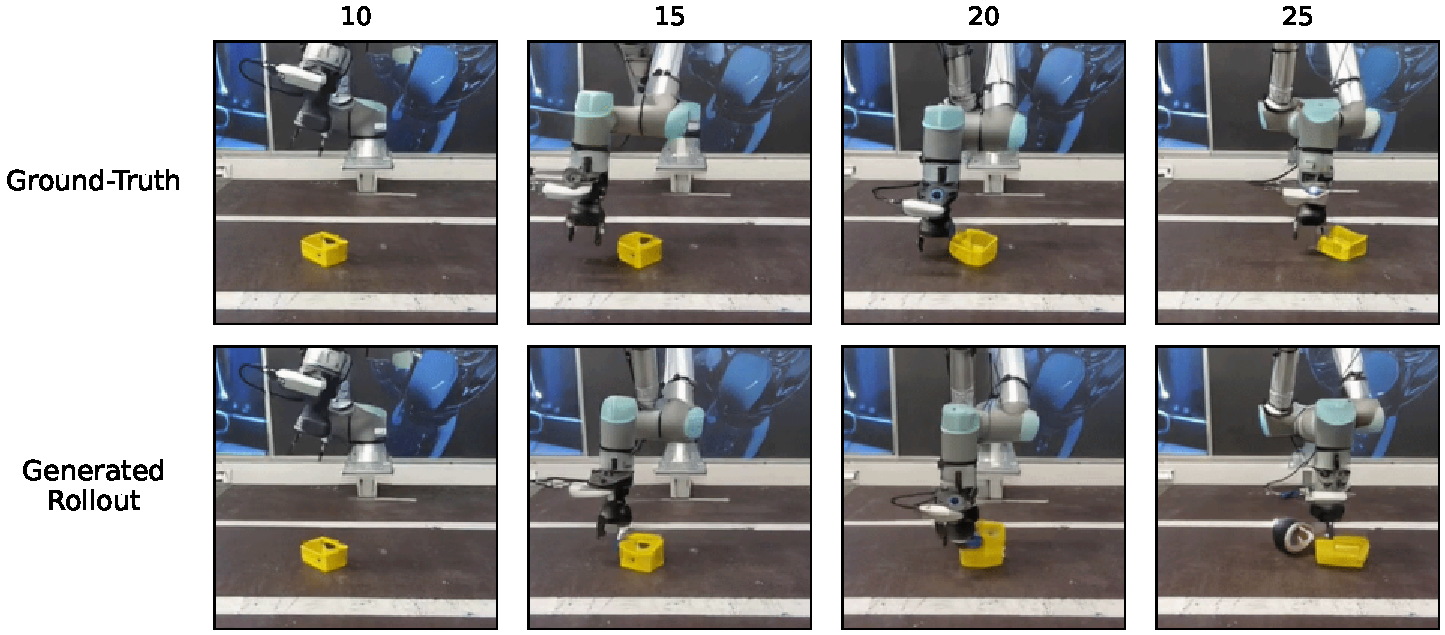
\includegraphics[width=1.0\textwidth]{images/comparison_2_part1.pdf}
    \\[2mm]
    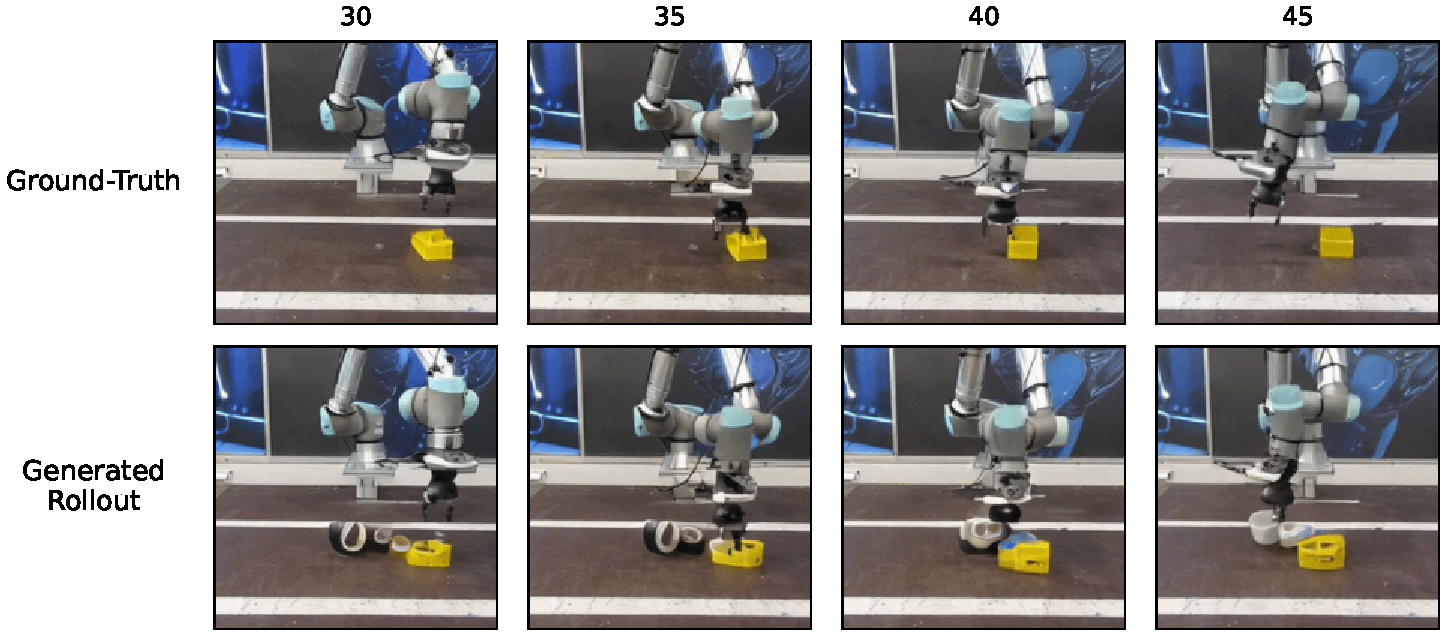
\includegraphics[width=1.0\textwidth]{images/comparison_2_part2.pdf}
    \caption{Additional qualitative rollout example on a held-out UR5 sequence.}
    \label{fig:appendix-rollout-example-2}
\end{figure}

\begin{figure}[H]
    \centering
    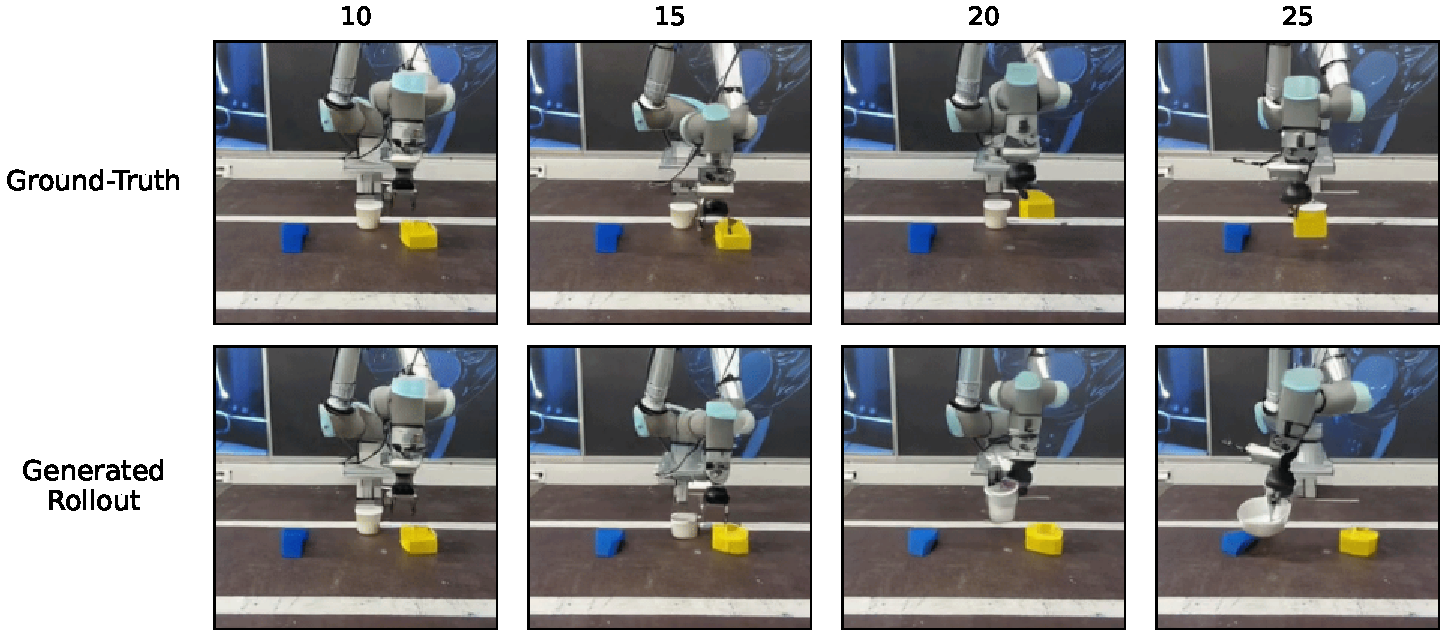
\includegraphics[width=1.0\textwidth]{images/comparison_6_part1.pdf}
    \\[2mm]
    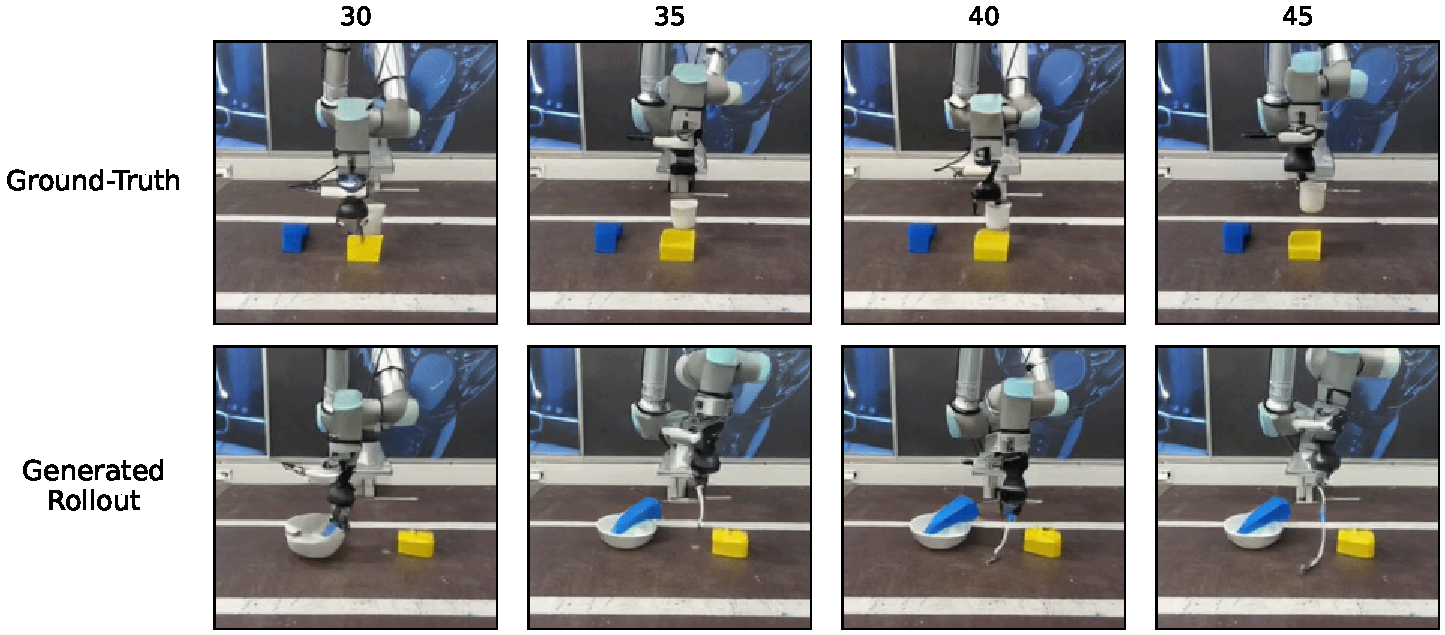
\includegraphics[width=1.0\textwidth]{images/comparison_6_part2.pdf}
    \caption{Additional qualitative rollout example on a held-out UR5 sequence.}
    \label{fig:appendix-rollout-example-6}
\end{figure}

\begin{figure}[H]
    \centering
    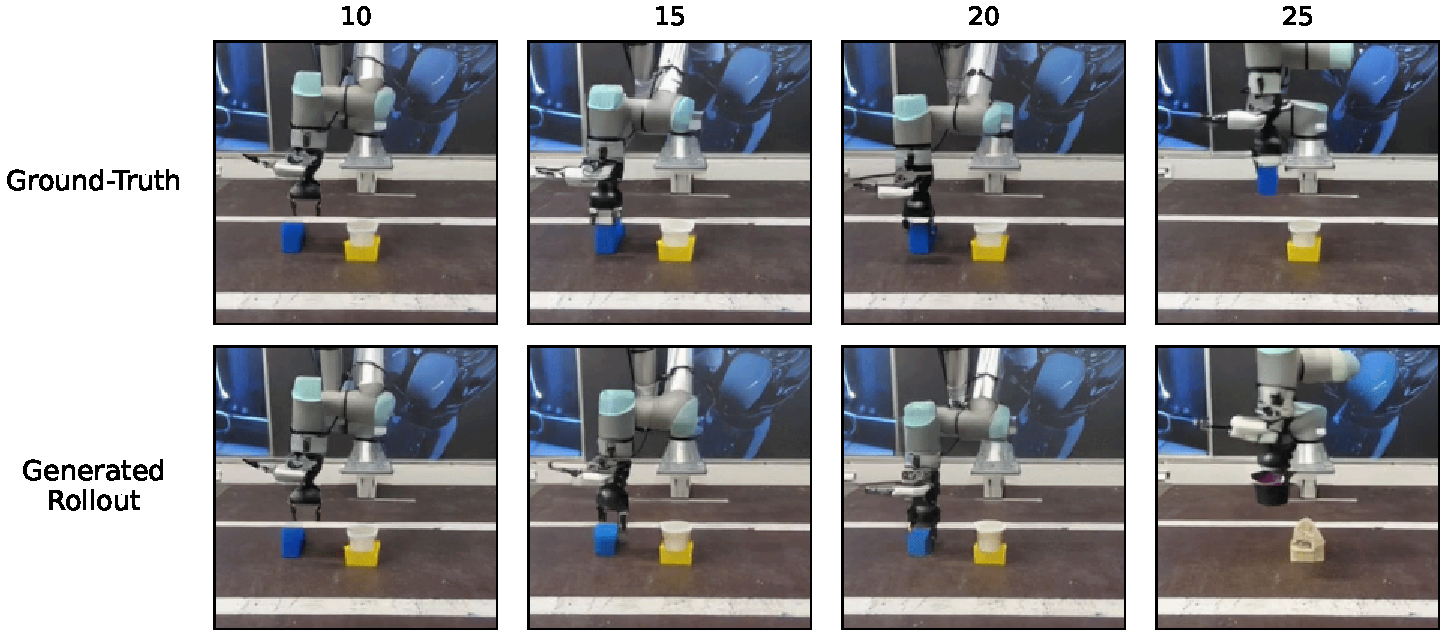
\includegraphics[width=1.0\textwidth]{images/comparison_7_part1.pdf}
    \\[2mm]
    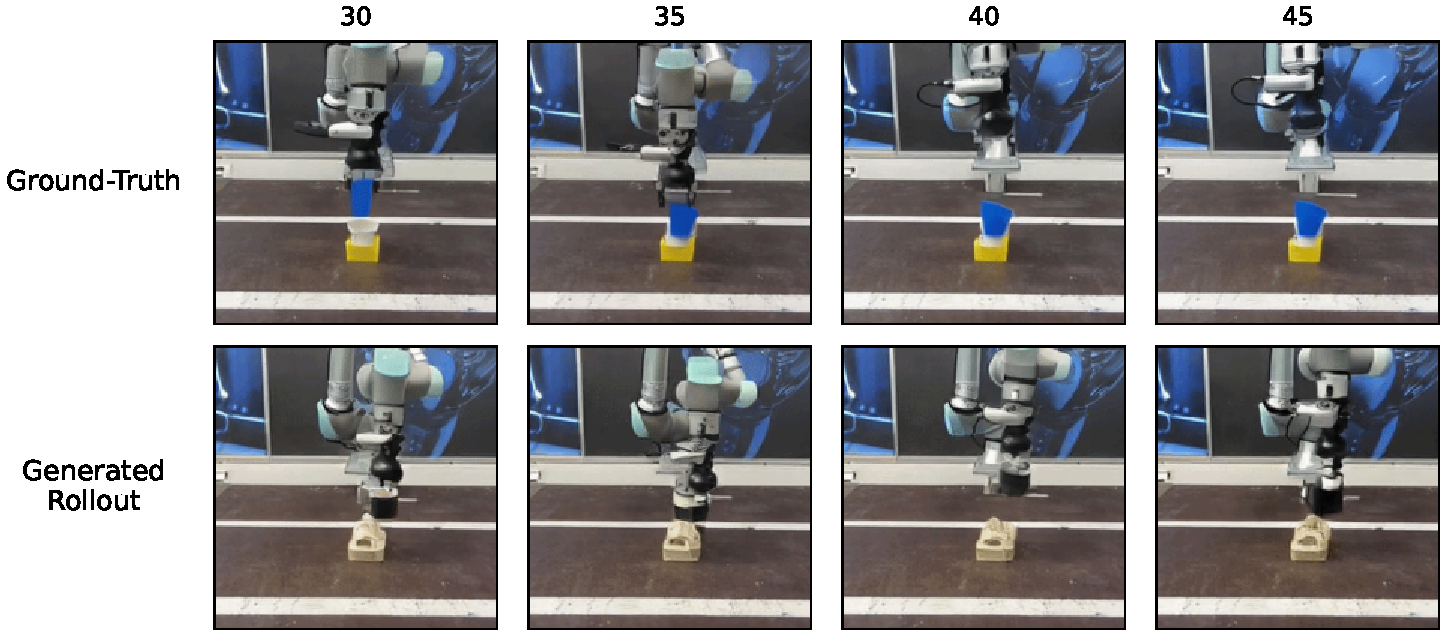
\includegraphics[width=1.0\textwidth]{images/comparison_7_part2.pdf}
    \caption{Additional qualitative rollout example on a held-out UR5 sequence.}
    \label{fig:appendix-rollout-example-7}
\end{figure}

\newpage

%%=== License ===
\chapter*{Non-exclusive licence to reproduce the thesis and make the thesis public}
\addcontentsline{toc}{chapter}{Non-exclusive licence}
\thispagestyle{empty}

I, Gauthier Bassereau,
\begin{enumerate}
\item grant the University of Tartu a free permit (non-exclusive licence) to reproduce, for the purpose of preservation, including for adding to the digital archives of the University of Tartu until the expiry of the term of copyright, my thesis
\begin{center}
\textbf{``Diffusion World Model for Robotics''},
\end{center}
supervised by Karl Kruusamäe and Agnes Luhtaru;
\item grant the University of Tartu the permit to make the thesis specified in point 1 available to the public via the web environment of the University of Tartu, including via the digital archives, under the Creative Commons licence CC BY NC ND 4.0, which allows, by giving appropriate credit to Gauthier Bassereau, to reproduce, distribute the work and communicate it to the public, and prohibits the creation of derivative works and any commercial use of the work from 31/12/2026 until the expiry of the term of copyright;
\item am aware that Gauthier Bassereau retains the rights specified in points 1 and 2;
\item confirm that granting the non-exclusive licence does not infringe other persons' intellectual property rights or rights arising from the personal data protection legislation.
\end{enumerate}
\vspace{2cm}
\textit{Gauthier Bassereau}
\\
\textbf{20/05/2026}
\end{document}
